\documentclass[12pt,a4paper,oneside]{report}

% --- Packages ---
\usepackage[utf8]{inputenc}
\usepackage[margin=1in]{geometry}
\usepackage{setspace}
\onehalfspacing

\usepackage{amsmath,amssymb,amsfonts,amsthm}
\usepackage{graphicx}
\graphicspath{{figures/}}
\usepackage{booktabs}
\usepackage{tabularx}
\usepackage{caption}
\usepackage{subcaption}
\usepackage{cite}
\usepackage{microtype}
\usepackage{xcolor}
\usepackage{fancyhdr}
\usepackage{titlesec}
\usepackage{listings}

\usepackage[colorlinks=true,linkcolor=blue!70!black,citecolor=green!50!black,urlcolor=magenta!70!black]{hyperref}

% --- Code Listing Style ---
\lstset{
  basicstyle=\ttfamily\footnotesize,
  backgroundcolor=\color{gray!8},
  frame=single,
  breaklines=true,
  keywordstyle=\color{blue}\bfseries,
  commentstyle=\color{green!60!black}\itshape,
  stringstyle=\color{red!70!black},
  numbers=left,
  numberstyle=\tiny\color{gray},
  stepnumber=1,
  tabsize=2
}

% --- Header and Footer ---
\pagestyle{fancy}
\fancyhf{}
\fancyhead[L]{\nouppercase{\leftmark}}
\fancyhead[R]{\thepage}
\renewcommand{\headrulewidth}{0.4pt}

% --- Chapter Title Formatting ---
\titleformat{\chapter}[display]
  {\normalfont\huge\bfseries}{\chaptertitlename\ \thechapter}{18pt}{\Huge}
\titlespacing*{\chapter}{0pt}{20pt}{20pt}

\begin{document}

% ==========================================
% TITLE PAGE
% ==========================================
\begin{titlepage}
\begin{center}
    \vspace*{0.5cm}
    
    {\Large \textbf{PROJECT REPORT}}\\[0.4cm]
    {\large \textbf{CSP 1602: Multivariate Statistical Analysis}}\\[1.2cm]
    
    \rule{\linewidth}{1.2pt}\\[0.4cm]
    {\LARGE \bfseries Statistical Characterisation of Sparse Activations and Low-Rank Latent Structures in Dense Feed-Forward Neural Networks}\\[0.2cm]
    \rule{\linewidth}{1.2pt}\\[1.5cm]
    
    \textit{Submitted by}\\[0.3cm]
    \textbf{Lakshmi Ganapathi Kodi} \quad (Roll No.: BT23MA005)\\[0.15cm]
    \textbf{Saurabh Kumar Guptha} \quad (Roll No.: BT23MA006)\\[0.4cm]
    \textit{Semester: 7}\\[1.8cm]
    
    \textit{Under the guidance of}\\[0.3cm]
    \textbf{Dr. C Lalengmawia}\\[0.1cm]
    Assistant Professor, Department of CSE\\[0.1cm]
    National Institute of Technology Mizoram\\[1.8cm]
    
    \vfill
    
    \begin{figure}[h]
        \centering
        % Department Details
    \end{figure}
    
    \textbf{Department of Computer Science \& Engineering}\\
    \textbf{National Institute of Technology Mizoram}\\
    Aizawl -- 796012, Mizoram, India\\[0.3cm]
    \textbf{November 2026}
\end{center}
\end{titlepage}

% ==========================================
% ABSTRACT
% ==========================================
\pagenumbering{roman}
\setcounter{page}{2}

\chapter*{Abstract}
\addcontentsline{toc}{chapter}{Abstract}

Feed-forward neural network (FFN) sub-layers contain the vast majority of learned parameters in modern Transformer-based causal language models. Although parameter matrices are entirely dense, non-linear activation functions such as ReLU frequently set intermediate features to exact zero. This study provides an end-to-end multivariate statistical characterisation of intermediate post-ReLU activations across all 12 layers of OPT-125M evaluated on the WikiText-2 benchmark.

We formulate and test five foundational multivariate research questions. First, repeated-measures ANOVA, Greenhouse-Geisser sphericity adjustment ($\hat{\epsilon} = 0.125, p < 10^{-45}$), and non-parametric Friedman tests ($Q = 432.99, p < 10^{-85}$) decisively reject profile flatness across network depth, identifying a dramatic early-intermediate sparsity spike where Layer~3 reaches 98.77\% exact zeros. Second, prevalence-filtered neuron co-activation analysis reveals strong positive clusters in early layers ($\text{mean } \phi = 0.068$) transitioning into near-orthogonal, independent detectors in intermediate layers ($\text{median } \phi \approx -0.01$). Third, covariance-based PCA and Roy-Vetterli spectral entropy effective rank quantify severe latent collapse: Layer~0 operates with an effective rank of merely $1.51$ ($>80\%$ variance in 1 component), while middle layers expand to approximately $46$ effective dimensions with over 90\% split-half subspace stability. Fourth, SVD on incoming and outgoing weight matrices of frozen OPT-125M reveals that parameter dimensionality strongly couples with activation dimensionality across depth ($r = 0.799, p = 0.0018$; Spearman $\rho = 0.839, p = 0.0006$), showing that early layer activation bottlenecks are directly underpinned by lower parameter capacity ($\text{mean } \text{erank}_W = 500.53$). Finally, evaluation across genuine text domains (Wikipedia, ML-ArXiv, and AG-News) via One-Way MANOVA decisively rejects domain profile equality (Wilks' $\Lambda = 0.6939$, Rao's $F(16, 5980) = 74.94, p < 10^{-200}$), with cross-validated Linear Discriminant Analysis achieving $55.83\%$ 3-class accuracy (relative to a $33.33\%$ chance baseline), confirming domain-specific semantic encoding.

\vspace{0.8cm}
\noindent \textbf{Keywords:} Activation Sparsity, Transformer Feed-Forward Networks, Multivariate Statistical Analysis, Profile Analysis, Effective Rank, MANOVA, Discriminant Analysis.

% ==========================================
% ACKNOWLEDGEMENTS
% ==========================================
\chapter*{Acknowledgements}
\addcontentsline{toc}{chapter}{Acknowledgements}

We express our deepest sense of gratitude to our project supervisor, \textbf{Dr. C Lalengmawia}, Assistant Professor, Department of Computer Science \& Engineering, National Institute of Technology Mizoram, for his continuous encouragement, insightful guidance, and constructive feedback throughout the course of this investigation.

We would also like to thank the faculty members and laboratory staff of the Department of Computer Science \& Engineering and the Department of Mathematics for providing the computational resources, foundational academic training, and collaborative research environment necessary to bring this multivariate statistical investigation to completion. Finally, we thank our peers and families for their unfailing patience and support.

\vspace{1.5cm}
\begin{flushright}
\textbf{Lakshmi Ganapathi Kodi} (BT23MA005)\\
\textbf{Saurabh Kumar Guptha} (BT23MA006)\\[0.2cm]
\textit{National Institute of Technology Mizoram}\\
\textit{November 2026}
\end{flushright}

% ==========================================
% TOC, LIST OF FIGURES, LIST OF TABLES
% ==========================================
\tableofcontents
\listoffigures
\listoftables

\clearpage
\pagenumbering{arabic}
\setcounter{page}{1}

% ==========================================
% CHAPTER 1: INTRODUCTION
% ==========================================
\chapter{Introduction}
\label{ch:intro}

\section{Background and Context}
Large Language Models (LLMs) built on the autoregressive Transformer architecture dominate contemporary artificial intelligence, achieving remarkable natural language generation and reasoning capabilities. A standard decoder-only Transformer block interleaves multi-head causal self-attention with position-wise Feed-Forward Networks (FFNs). While attention heads dynamically route contextual information across different token positions, FFN sub-layers perform point-wise non-linear feature transformations at every single sequence position.

In models such as Meta's Open Pre-trained Transformers (OPT), the FFN sub-layer expands token representations from a hidden embedding dimension ($d_{\text{model}} = 768$) to a wide intermediate dimension ($d_{\text{ffn}} = 3072$) through a first linear projection ($\text{fc1}$), applies a non-linear activation function ($\text{ReLU}$), and projects back to the residual stream through a second linear transformation ($\text{fc2}$). Crucially, FFN layers contain approximately two-thirds of the total parameter count in non-embedding Transformer layers. 

Recent theoretical work interprets FFN layers as key-value associative memories \cite{geva2021transformer}: the first matrix ($\text{fc1}$) projects input token representations onto keys that detect semantic or syntactic patterns, while the second matrix ($\text{fc2}$) writes corresponding value vectors into the residual representation. Despite the weight matrices being dense and unconstrained during training, the non-linear activation function enforces exact zero values for all negative pre-activations. As a consequence, only a fraction of the 3,072 neurons activate for any given token, a phenomenon termed \textit{activation sparsity} \cite{li2023emergence}.

\section{Problem Statement}
Although activation sparsity has recently drawn attention in machine learning systems for computational acceleration, the underlying statistical geometry of these activations remains largely uncharacterized. In particular, four critical questions remain open:
\begin{enumerate}
    \item Does activation sparsity remain constant across network depth, or do early, middle, and late Transformer layers operate under statistically distinguishable sparsity regimes?
    \item Do intermediate neurons fire as mutually independent feature detectors, or do they exhibit pronounced pairwise statistical dependence and functional clustering?
    \item Can the high-dimensional variation of 3,072 intermediate neurons be represented by a compact, lower-dimensional latent subspace, and how does this effective dimensionality evolve across layers?
    \item Is the observed dimensionality of activation representations bounded by the static singular spectrum of the FFN weight matrices, or is it dynamically shaped by the data distribution?
    \item How invariant are these activation distributions when the neural network is exposed to text from divergent linguistic domains?
\end{enumerate}
Addressing these questions requires moving beyond scalar summaries to formal \textit{multivariate statistical analysis} (MVS), treating token activations as high-dimensional random vectors.

\section{Research Objectives}
This project systematically investigates the activation behaviour of the 12 FFN layers in frozen OPT-125M on WikiText-2. Specifically, we define five core research questions (RQs) directly derived from our approved project proposal:
\begin{itemize}
    \item \textbf{Objective 1 (RQ1): Layer-wise Sparsity Profile Analysis.} Formulate text blocks as multivariate repeated-measure units and perform profile flatness tests, Repeated-Measures ANOVA with Greenhouse-Geisser corrections, and the non-parametric Friedman test.
    \item \textbf{Objective 2 (RQ2): Statistical Neuron Dependence.} Construct joint, marginal, and conditional empirical probability distributions, estimate binary-indicator $\phi$-correlation matrices, and perform hierarchical agglomerative clustering across layers.
    \item \textbf{Objective 3 (RQ3): Latent Dimensionality and Factor Structure.} Apply covariance-based Principal Component Analysis (PCA), compute Participation Ratios ($\text{PR}$) and Roy-Vetterli spectral entropy effective ranks ($\text{erank}$), evaluate split-half subspace stability, and fit exploratory Gaussian factor models.
    \item \textbf{Objective 4 (RQ4): Activation versus Weight Dimensionality.} Extract incoming and outgoing FFN weight matrices ($\text{fc1}, \text{fc2}$), compute their SVD singular spectra, and evaluate rank correlation against empirical activation effective dimensionality.
    \item \textbf{Objective 5 (RQ5): Cross-Domain Representation Stability.} Assess activation stability across three distinct text domains (Wikipedia, Scientific, News) using two-sample Hotelling's $T^2$ tests, One-Way MANOVA, Box's M equality of covariance test, and Linear Discriminant Analysis (LDA).
\end{itemize}

\section{Scope and Methodological Delimitations}
\begin{itemize}
    \item \textbf{Exact Target Activation Point:} Activations are captured strictly \textit{post-ReLU and pre-$\text{fc2}$}. Because $\text{ReLU}(z) = \max(0, z)$, zero values are mathematically exact zeros, eliminating arbitrary thresholding heuristics.
    \item \textbf{Sampling Unit Discipline:} Neighboring tokens within a sentence or document exhibit local temporal autocorrelation. Consequently, formal hypothesis testing in RQ1 uses independent 128-token text blocks as the sampling units rather than treating adjacent tokens as independent replicates.
    \item \textbf{Dimensionality Conditioning:} Because the intermediate dimension ($p = 3072$) exceeds token batch sample sizes in exploratory tests, dimensionality reduction via PCA is leveraged to guarantee full-rank, well-conditioned covariance matrices before running MANOVA and Hotelling's $T^2$ tests.
\end{itemize}

\section{Organisation of the Report}
The remainder of this report is structured as follows: Chapter~\ref{ch:lit_review} provides the theoretical literature review and mathematical foundations of the multivariate statistical methods employed. Chapter~\ref{ch:methodology} describes the software engineering architecture, activation extraction pipeline, and mathematical formulations for each research question. Chapter~\ref{ch:results} details the empirical results, figures, tables, and statistical interpretations for RQ1 through RQ5. Chapter~\ref{ch:conclusion} concludes with principal findings, practical implications for neural network pruning, and future directions.

% ==========================================
% CHAPTER 2: LITERATURE REVIEW & THEORY
% ==========================================
\chapter{Literature Review and Theoretical Foundations}
\label{ch:lit_review}

\section{Feed-Forward Networks as Key-Value Memories}
In a Transformer decoder block, the token representation $\mathbf{x} \in \mathbb{R}^{d_{\text{model}}}$ is passed to the FFN sub-layer. In OPT-125M, the computation is governed by:
\begin{equation}
    \label{eq:ffn_formulation}
    \mathbf{h} = \text{ReLU}(\mathbf{x} \mathbf{W}_1 + \mathbf{b}_1), \qquad \mathbf{y} = \mathbf{h} \mathbf{W}_2 + \mathbf{b}_2
\end{equation}
where $\mathbf{W}_1 \in \mathbb{R}^{d_{\text{model}} \times d_{\text{ffn}}}$, $\mathbf{b}_1 \in \mathbb{R}^{d_{\text{ffn}}}$, $\mathbf{W}_2 \in \mathbb{R}^{d_{\text{ffn}} \times d_{\text{model}}}$, and $\mathbf{b}_2 \in \mathbb{R}^{d_{\text{model}}}$. Geva et al.\ \cite{geva2021transformer} demonstrated that the column vectors of $\mathbf{W}_1$ act as pattern detectors or \textit{keys}, firing when the input vector $\mathbf{x}$ matches specific n-gram or topical triggers. The corresponding row vectors of $\mathbf{W}_2$ act as \textit{values}, injecting learned concepts into the next token prediction distribution. Because knowledge retrieval in language models requires selective factual triggering, only a sparse subset of keys should activate for any given context.

\section{Emergence of Activation Sparsity}
Li et al.\ \cite{li2023emergence} showed that activation sparsity naturally emerges during Transformer pre-training with ReLU activations without explicit $L_1$ regularization. In massive models, over 80\% to 95\% of intermediate neurons output exact zero on typical text. Understanding whether this sparsity is uniformly distributed across layers or concentrated in specific processing stages is crucial for both theoretical interpretability and modern sparse-inference serving frameworks.

\section{Multivariate Statistical Methodology}

\subsection{Random Vectors and Sample Moments}
Let $\mathbf{h} = [h_1, h_2, \dots, h_p]^T \in \mathbb{R}^p$ represent the $p$-dimensional random vector of intermediate activations ($p = 3072$). For a sample of $n$ observations, the sample mean vector $\bar{\mathbf{h}}$ and sample covariance matrix $\mathbf{S}$ are defined as:
\begin{equation}
    \label{eq:sample_moments}
    \bar{\mathbf{h}} = \frac{1}{n} \sum_{i=1}^n \mathbf{h}_i, \qquad \mathbf{S} = \frac{1}{n - 1} \sum_{i=1}^n (\mathbf{h}_i - \bar{\mathbf{h}})(\mathbf{h}_i - \bar{\mathbf{h}})^T
\end{equation}

\subsection{Profile Analysis and Repeated-Measures ANOVA}
Profile analysis is the multivariate analogue of repeated-measures ANOVA, designed for situations where $p$ repeated measurements (here, sparsity across 12 layers) are collected on $n$ independent subjects (text blocks) \cite{johnson2014applied}. 
Let $\mathbf{y}_i = [y_{i1}, y_{i2}, \dots, y_{ip}]^T \in \mathbb{R}^p$ denote the block-averaged sparsity vector for block $i$. The null hypothesis of \textit{profile flatness} posits that the layer mean sparsity is identical across all layers:
\begin{equation}
    \label{eq:rq1_flatness_hypothesis}
    H_0: \mu_1 = \mu_2 = \dots = \mu_p \quad \iff \quad H_0: \mathbf{C} \boldsymbol{\mu} = \mathbf{0} \quad \text{(RQ1)}
\end{equation}
where $\mathbf{C} \in \mathbb{R}^{(p-1) \times p}$ is a contrast matrix subtracting the reference layer ($\mu_1$) from subsequent layers:
\begin{equation}
    \label{eq:rq1_contrast_matrix}
    \mathbf{C} = \begin{bmatrix}
        -1 & 1 & 0 & \dots & 0\\
        -1 & 0 & 1 & \dots & 0\\
        \vdots & \vdots & \vdots & \ddots & \vdots\\
        -1 & 0 & 0 & \dots & 1
    \end{bmatrix} \quad \text{(RQ1)}
\end{equation}
The contrast sample mean and covariance are $\bar{\mathbf{d}} = \mathbf{C} \bar{\mathbf{y}}$ and $\mathbf{S}_d = \mathbf{C} \mathbf{S} \mathbf{C}^T$. The one-sample Hotelling's $T^2$ statistic is:
\begin{equation}
    \label{eq:rq1_hotelling}
    T^2 = n \bar{\mathbf{d}}^T \mathbf{S}_d^{-1} \bar{\mathbf{d}} \quad \text{(RQ1)}
\end{equation}
which transforms under the null hypothesis to an exact $F$-distribution:
\begin{equation}
    \label{eq:rq1_f_trans}
    F = \frac{n - (p - 1)}{(p - 1)(n - 1)} T^2 \sim F(p - 1, \, n - p + 1) \quad \text{(RQ1)}
\end{equation}
When the sphericity assumption of repeated-measures ANOVA is violated, the Greenhouse-Geisser adjustment factor $\hat{\epsilon}$ modifies the degrees of freedom:
\begin{equation}
    \label{eq:rq1_gg_epsilon}
    \hat{\epsilon} = \frac{[\text{tr}(\mathbf{S}_d)]^2}{(p - 1) \, \text{tr}(\mathbf{S}_d^2)} \quad \text{(RQ1)}
\end{equation}
where $\hat{\epsilon} \in [1/(p-1), 1]$. The non-parametric Friedman test evaluates rank consistency across blocks without normality assumptions:
\begin{equation}
    \label{eq:rq1_friedman}
    Q = \frac{12}{n p (p + 1)} \sum_{j=1}^p R_j^2 - 3 n (p + 1) \sim \chi^2(p - 1) \quad \text{(RQ1)}
\end{equation}
where $R_j$ is the sum of ranks for layer $j$ across the $n$ blocks.

\subsection{Measures of Effective Dimensionality}
In high-dimensional activation analysis, counting components that cross an arbitrary variance threshold (e.g., 80\%) is sensitive to discretization. We implement two continuous, invariant measures of effective dimensionality based on the eigenvalues $\lambda_1 \ge \lambda_2 \ge \dots \ge \lambda_m$ of the covariance matrix $\mathbf{S}$.

\paragraph{Participation Ratio ($\text{PR}$):} Defined from statistical physics and neural coding as:
\begin{equation}
    \label{eq:rq3_participation_ratio}
    \text{PR} = \frac{\left( \sum_{i=1}^m \lambda_i \right)^2}{\sum_{i=1}^m \lambda_i^2} = \frac{[\text{tr}(\mathbf{S})]^2}{\text{tr}(\mathbf{S}^2)} = \frac{[\text{tr}(\mathbf{S})]^2}{\|\mathbf{S}\|_F^2} \quad \text{(RQ3)}
\end{equation}
If all variance is concentrated along a single dimension ($\lambda_1 > 0, \lambda_{i>1} = 0$), $\text{PR} = 1$. If variance is uniformly isotropic ($\lambda_1 = \dots = \lambda_m$), $\text{PR} = m$.

\paragraph{Spectral Entropy Effective Rank ($\text{erank}$):} Formulated by Roy and Vetterli \cite{roy2007effective}, the spectral probability distribution is $p_i = \lambda_i / \sum_{j=1}^m \lambda_j$. The effective rank is the exponential of the Shannon spectral entropy:
\begin{equation}
    \label{eq:rq3_erank}
    H = -\sum_{i=1}^m p_i \ln p_i, \qquad \text{erank} = \exp(H) \quad \text{(RQ3)}
\end{equation}
Effective rank provides a smooth, mathematically principled measure of dimensional complexity on the scale $[1, m]$.

\subsection{Multivariate Analysis of Variance (MANOVA) and Discriminant Analysis}
To evaluate whether mean activation vectors remain statistically invariant across $G = 3$ text domains (RQ5), One-Way MANOVA partitions the total sum of squares and cross-products matrix $\mathbf{T}$ into between-domain hypothesis ($\mathbf{H}$) and within-domain error ($\mathbf{E}$) matrices \cite{hardle2019applied}:
\begin{equation}
    \label{eq:rq5_manova_he}
    \mathbf{H} = \sum_{g=1}^G n_g (\bar{\mathbf{x}}_g - \bar{\mathbf{x}})(\bar{\mathbf{x}}_g - \bar{\mathbf{x}})^T, \qquad \mathbf{E} = \sum_{g=1}^G \sum_{i=1}^{n_g} (\mathbf{x}_{gi} - \bar{\mathbf{x}}_g)(\mathbf{x}_{gi} - \bar{\mathbf{x}}_g)^T \quad \text{(RQ5)}
\end{equation}
The four classical test criteria are derived from the eigenvalues $\xi_1 \ge \xi_2 \dots \ge \xi_s$ of $\mathbf{E}^{-1}\mathbf{H}$:
\begin{align}
    \label{eq:rq5_manova_criteria}
    \text{Wilks' Lambda:} \quad \Lambda &= \prod_{i=1}^s \frac{1}{1 + \xi_i} = \frac{\det(\mathbf{E})}{\det(\mathbf{H} + \mathbf{E})} \quad \text{(RQ5)}\\
    \text{Pillai's Trace:} \quad V &= \sum_{i=1}^s \frac{\xi_i}{1 + \xi_i} = \text{tr}(\mathbf{H}(\mathbf{H} + \mathbf{E})^{-1}) \quad \text{(RQ5)}\\
    \text{Hotelling-Lawley Trace:} \quad U &= \sum_{i=1}^s \xi_i = \text{tr}(\mathbf{E}^{-1}\mathbf{H}) \quad \text{(RQ5)}\\
    \text{Roy's Largest Root:} \quad \theta &= \frac{\xi_1}{1 + \xi_1} \quad \text{(RQ5)}
\end{align}
Rao's $F$-approximation converts Wilks' $\Lambda$ into an exact or approximate $F$-statistic to test $H_0: \boldsymbol{\mu}_1 = \boldsymbol{\mu}_2 = \boldsymbol{\mu}_3$.

To test whether domain covariance structures are identical ($H_0: \boldsymbol{\Sigma}_1 = \boldsymbol{\Sigma}_2 = \boldsymbol{\Sigma}_3$), Box's M statistic is given by:
\begin{equation}
    \label{eq:rq5_box_m}
    M = (N - G) \ln |\mathbf{S}_{\text{pooled}}| - \sum_{g=1}^G (n_g - 1)\ln|\mathbf{S}_g| \quad \text{(RQ5)}
\end{equation}

% ==========================================
% CHAPTER 3: METHODOLOGY
% ==========================================
\chapter{Methodology and System Architecture}
\label{ch:methodology}

\section{System Architecture}
The experimental framework is implemented as an extensible Python package (`sparse_ffn`) structured into decoupled pipelines for data processing, activation extraction, multivariate statistical testing, and automated reporting.

\begin{figure}[h]
    \centering
    \fbox{\parbox{0.92\linewidth}{
    \centering
    \textbf{System Architecture Pipeline}\\[0.3cm]
    \texttt{Hugging Face WikiText-2 Benchmark}\\
    $\Downarrow$\\
    \texttt{Tokenization \& Chunking (L=128, EOS Preservation) $\to$ data/processed/wikitext2/}\\
    $\Downarrow$\\
    \texttt{Frozen OPT-125M Forward Hook (Post-ReLU, Pre-fc2) $\to$ artifacts/activations/}\\
    $\Downarrow$\\
    \begin{tabular}{ccccc}
        \textbf{RQ1 Engine} & \textbf{RQ2 Engine} & \textbf{RQ3 Engine} & \textbf{RQ4 Engine} & \textbf{RQ5 Engine}\\
        RM-ANOVA & $\phi$-Corr \& Cluster & PCA \& erank & SVD Weight Rank & MANOVA \& LDA\\
    \end{tabular}\\
    $\Downarrow$\\
    \texttt{Artifacts Archive (CSVs, High-Resolution Plots, JSON Reports)}
    }}
    \caption{End-to-end data processing and multivariate statistical analysis architecture.}
    \label{fig:arch_diagram}
\end{figure}

\section{Data Pipeline and Token Chunking}
We utilize the official `Salesforce/wikitext` (`wikitext-2-raw-v1`) corpus. Rather than randomly slicing text strings, non-empty text rows are encoded using the official byte-pair encoding (BPE) tokenizer for OPT-125M. The end-of-sequence token ($\langle\text{s}\rangle$, ID 2) is explicitly appended to every source document row to delineate semantic boundaries before sequential stream concatenation. The concatenated sequence is partitioned into non-overlapping contiguous blocks of length $L = 128$. The final shorter block is preserved. Padding positions are tracked via `attention_mask` and strictly filtered out during activation extraction, ensuring that all analyzed activation rows correspond to genuine text tokens.

\section{Activation Extraction Mechanics}
The OPT-125M architecture comprises 12 Transformer decoder layers. For each layer $\ell \in \{0, 1, \dots, 11\}$, intermediate representations are extracted by registering forward hooks directly on the activation module:
\begin{equation}
    \label{eq:extraction_hook}
    \mathbf{h}^{(\ell)} = \text{ReLU}\left( \text{fc1}^{(\ell)}(\mathbf{x}^{(\ell)}) \right) \in \mathbb{R}^{B \times L \times 3072}
\end{equation}
Hooked activations are filtered for non-padding tokens, cast to 16-bit floating point (`float16`), and sharded to compressed `.npz` archives alongside integer metadata arrays recording token block IDs (`block_ids`) and within-block sequence offsets (`token_positions`). Storing exact zeros in float16 incurs zero numerical degradation. A pilot extraction comprising 20 batches (5,120 valid tokens across 40 distinct text blocks) yields complete archives for all 12 layers.

\section{Mathematical Formulations for Research Questions}

\subsection{RQ1: Profile Flatness and Repeated-Measures ANOVA}
For each block $i \in \{1, \dots, n\}$ and layer $j \in \{1, \dots, p\}$, the block-averaged activation sparsity $s_{ij}$ is computed:
\begin{equation}
    \label{eq:rq1_block_sparsity}
    s_{ij} = \frac{1}{|B_i|} \sum_{t \in B_i} \frac{1}{d_{\text{ffn}}} \sum_{k=1}^{d_{\text{ffn}}} \mathbb{I}\left( h_{t,k}^{(j)} = 0 \right) \quad \text{(RQ1)}
\end{equation}
We evaluate the hypothesis of layer-wise sparsity flatness using contrast Hotelling's $T^2$ (Equation~\ref{eq:rq1_hotelling}, RQ1), Repeated-Measures ANOVA with Greenhouse-Geisser sphericity correction (Equation~\ref{eq:rq1_gg_epsilon}, RQ1), and Friedman's rank test (Equation~\ref{eq:rq1_friedman}, RQ1). Post-hoc pairwise comparisons between adjacent layers and against Layer~0 are evaluated with Holm-Bonferroni step-down correction.

\subsection{RQ2: Neuron Co-activation and Indicator Correlation}
For each neuron $k$, continuous post-ReLU activations are converted to binary active/inactive indicators:
\begin{equation}
    \label{eq:rq2_indicator}
    u_{t, k} = \mathbb{I}\left( h_{t, k} > 0 \right) \quad \text{(RQ2)}
\end{equation}
A prevalence filter is applied to exclude permanently dead or continuously active neurons:
\begin{equation}
    \label{eq:rq2_prevalence}
    \mathcal{K}_{\text{eligible}} = \left\{ k \;\middle|\; 0.01 \le \frac{1}{n}\sum_{t=1}^n u_{t,k} \le 0.99 \right\} \quad \text{(RQ2)}
\end{equation}
A reproducible subset of $m = 128$ neurons is sampled. For each pair $(i, j)$, marginal probabilities $p_i, p_j$, joint probability $p_{11} = P(u_i=1, u_j=1)$, and conditional probability $P(u_i=1 \mid u_j=1) = p_{11} / p_j$ are computed. The binary Pearson correlation (phi coefficient $\phi$) is given by:
\begin{equation}
    \label{eq:rq2_phi}
    \phi_{ij} = \frac{p_{11} - p_i p_j}{\sqrt{p_i (1 - p_i) p_j (1 - p_j)}} \quad \text{(RQ2)}
\end{equation}
Hierarchical agglomerative clustering is performed on correlation distance $d_{ij} = 1 - \phi_{ij}$ using average linkage.

\subsection{RQ3: PCA, Latent Dimensionality, and Sampling Stability}
Activations are centered (mean subtracted) but not variance-standardized, preserving the natural physical energy of neuron activations. PCA is fitted using randomized SVD. Effective dimensionality is evaluated via Participation Ratio (Equation~\ref{eq:rq3_participation_ratio}, RQ3) and Roy-Vetterli Entropy Rank (Equation~\ref{eq:rq3_erank}, RQ3).

To rigorously validate that discovered principal subspaces reflect genuine data geometry rather than finite-sample artifacts, we conduct split-half cross-validation. The $n$ tokens are randomly partitioned into two disjoint subsets $A$ and $B$ of size $n/2$. Independent PCA models are fitted to obtain top-$K$ orthonormal loading matrices $\mathbf{V}_A, \mathbf{V}_B \in \mathbb{R}^{p \times K}$. The singular values $\sigma_1 \ge \dots \ge \sigma_K$ of the cross-subspace projection matrix $\mathbf{M} = \mathbf{V}_A^T \mathbf{V}_B$ represent the cosines of the principal angles between the two subspaces. Subspace stability is quantified as:
\begin{equation}
    \label{eq:rq3_subspace_stability}
    \bar{\rho}_K = \frac{1}{K} \sum_{i=1}^K \sigma_i(\mathbf{V}_A^T \mathbf{V}_B) \in [0, 1] \quad \text{(RQ3)}
\end{equation}
Reconstruction error as a function of component count $K$ is tracked as:
\begin{equation}
    \label{eq:rq3_recon_error}
    \text{Error}(K) = 1 - \frac{\sum_{i=1}^K \lambda_i}{\sum_{i=1}^m \lambda_i} \quad \text{(RQ3)}
\end{equation}

\subsection{RQ4: Weight Matrix SVD versus Activation Dimensionality}
The FFN parameter matrices $\mathbf{W}_{\text{in}} \in \mathbb{R}^{3072 \times 768}$ ($\text{fc1}$) and $\mathbf{W}_{\text{out}} \in \mathbb{R}^{768 \times 3072}$ ($\text{fc2}$) are decomposed using Singular Value Decomposition:
\begin{equation}
    \label{eq:rq4_weight_svd}
    \mathbf{W} = \mathbf{U} \boldsymbol{\Sigma} \mathbf{V}^T, \qquad \boldsymbol{\Sigma} = \text{diag}(s_1, s_2, \dots, s_{768}) \quad \text{(RQ4)}
\end{equation}
Weight spectral energy is defined as $p_{i, W} = s_i^2 / \sum s_j^2$, yielding weight participation ratio $\text{PR}_W$ and entropy-based rank $\text{erank}_W$. We compute layer-wise Pearson correlation $r$ and Spearman rank correlation $\rho$ between activation effective rank $\text{erank}_A^{(\ell)}$ and mean weight rank $\text{erank}_W^{(\ell)}$ across all 12 layers:
\begin{equation}
    \label{eq:rq4_rank_corr}
    \rho = 1 - \frac{6 \sum_{i=1}^{12} d_i^2}{12(12^2 - 1)} \quad \text{(RQ4)}
\end{equation}

\subsection{RQ5: Cross-Domain Representation Testing}
To examine whether intermediate FFN representations remain invariant across text genres, we construct three distinct text domain representations: Wikipedia (factual/encyclopedic baseline), Scientific (technical lexicon and specialized co-activation), and News (event-driven narrative). Activations are projected to $K = 8$ common principal components (Step 8 of proposal) to satisfy non-singularity constraints ($N = 3000 \gg K = 8$). We compute pairwise Hotelling's $T^2$ tests (Equation~\ref{eq:rq1_hotelling}), One-Way MANOVA criteria (Equation~\ref{eq:rq5_manova_criteria}, RQ5), Box's M test (Equation~\ref{eq:rq5_box_m}, RQ5), and 5-fold cross-validated Linear Discriminant Analysis (LDA).

\section{Software Implementation and Test Verification}
The repository is engineered under strict software testing standards. Unit tests verify token chunking, padding masks, contrast matrices, eigenvalue calculations, SVD spectra, and MANOVA criteria using synthetic arrays. The test suite comprises 18 comprehensive tests executing under `pytest`.

% ==========================================
% CHAPTER 4: RESULTS AND DISCUSSION
% ==========================================
\chapter{Results and Discussion}
\label{ch:results}

\section{Phase 1: Descriptive Activation Sparsity Across Depth}
Table~\ref{tab:phase1_summary} summarizes the descriptive statistics of post-ReLU activations across all 12 layers of OPT-125M on the WikiText-2 validation tokens.

\begin{table}[h]
\centering
\small
\caption{Layer-wise descriptive summary of post-ReLU FFN activations.}
\label{tab:phase1_summary}
\begin{tabularx}{\linewidth}{lcccccc}
\toprule
\textbf{Layer} & \textbf{Zero Frac.} & \textbf{Mean Sparsity} & \textbf{Std Sparsity} & \textbf{Pos. Mean} & \textbf{Pos. Std} & \textbf{Pos. Skewness} \\
\midrule
Layer 00 & 0.8896 & 0.8896 & 0.0804 & 0.0600 & 0.2071 & 54.74 \\
Layer 01 & 0.9749 & 0.9749 & 0.0048 & 0.1032 & 0.1185 & 6.67 \\
Layer 02 & 0.9792 & 0.9792 & 0.0048 & 0.1118 & 0.2820 & 16.55 \\
Layer 03 & \textbf{0.9877} & \textbf{0.9877} & 0.0032 & 0.1112 & 0.1510 & 11.32 \\
Layer 04 & 0.9665 & 0.9665 & 0.0059 & 0.1092 & 0.1337 & 16.25 \\
Layer 05 & 0.9323 & 0.9323 & 0.0110 & 0.1047 & 0.0897 & 2.04 \\
Layer 06 & 0.9144 & 0.9144 & 0.0133 & 0.1073 & 0.0943 & 2.30 \\
Layer 07 & 0.9180 & 0.9180 & 0.0142 & 0.1191 & 0.1052 & 2.24 \\
Layer 08 & 0.9228 & 0.9228 & 0.0140 & 0.1446 & 0.1297 & 2.06 \\
Layer 09 & 0.9241 & 0.9241 & 0.0135 & 0.1754 & 0.1601 & 1.88 \\
Layer 10 & 0.9116 & 0.9116 & 0.0181 & 0.2087 & 0.1963 & 2.02 \\
Layer 11 & 0.9149 & 0.9149 & 0.0347 & \textbf{0.2517} & \textbf{0.3145} & 5.70 \\
\bottomrule
\end{tabularx}
\end{table}

The empirical zero fraction reveals three distinct architectural phases:
\begin{enumerate}
    \item \textbf{Input Filtering Phase (Layers 0--3):} Sparsity surges from 88.96\% in Layer~0 to a peak of 98.77\% in Layer~3. At Layer~3, the median neuron activation frequency is merely 0.058\%, meaning only approximately 38 out of 3,072 neurons fire for an average token.
    \item \textbf{Synthesizing Plateau Phase (Layers 4--10):} Sparsity stabilizes between 91.1\% and 93.2\%, accompanied by a steady upward trajectory in positive activation magnitude (positive mean rises from 0.109 to 0.209).
    \item \textbf{Output Readout Phase (Layer 11):} High magnitude activations emerge (positive mean: 0.2517, maximum std: 0.3145) with increased variance across token positions.
\end{enumerate}

\begin{figure}[h]
    \centering
    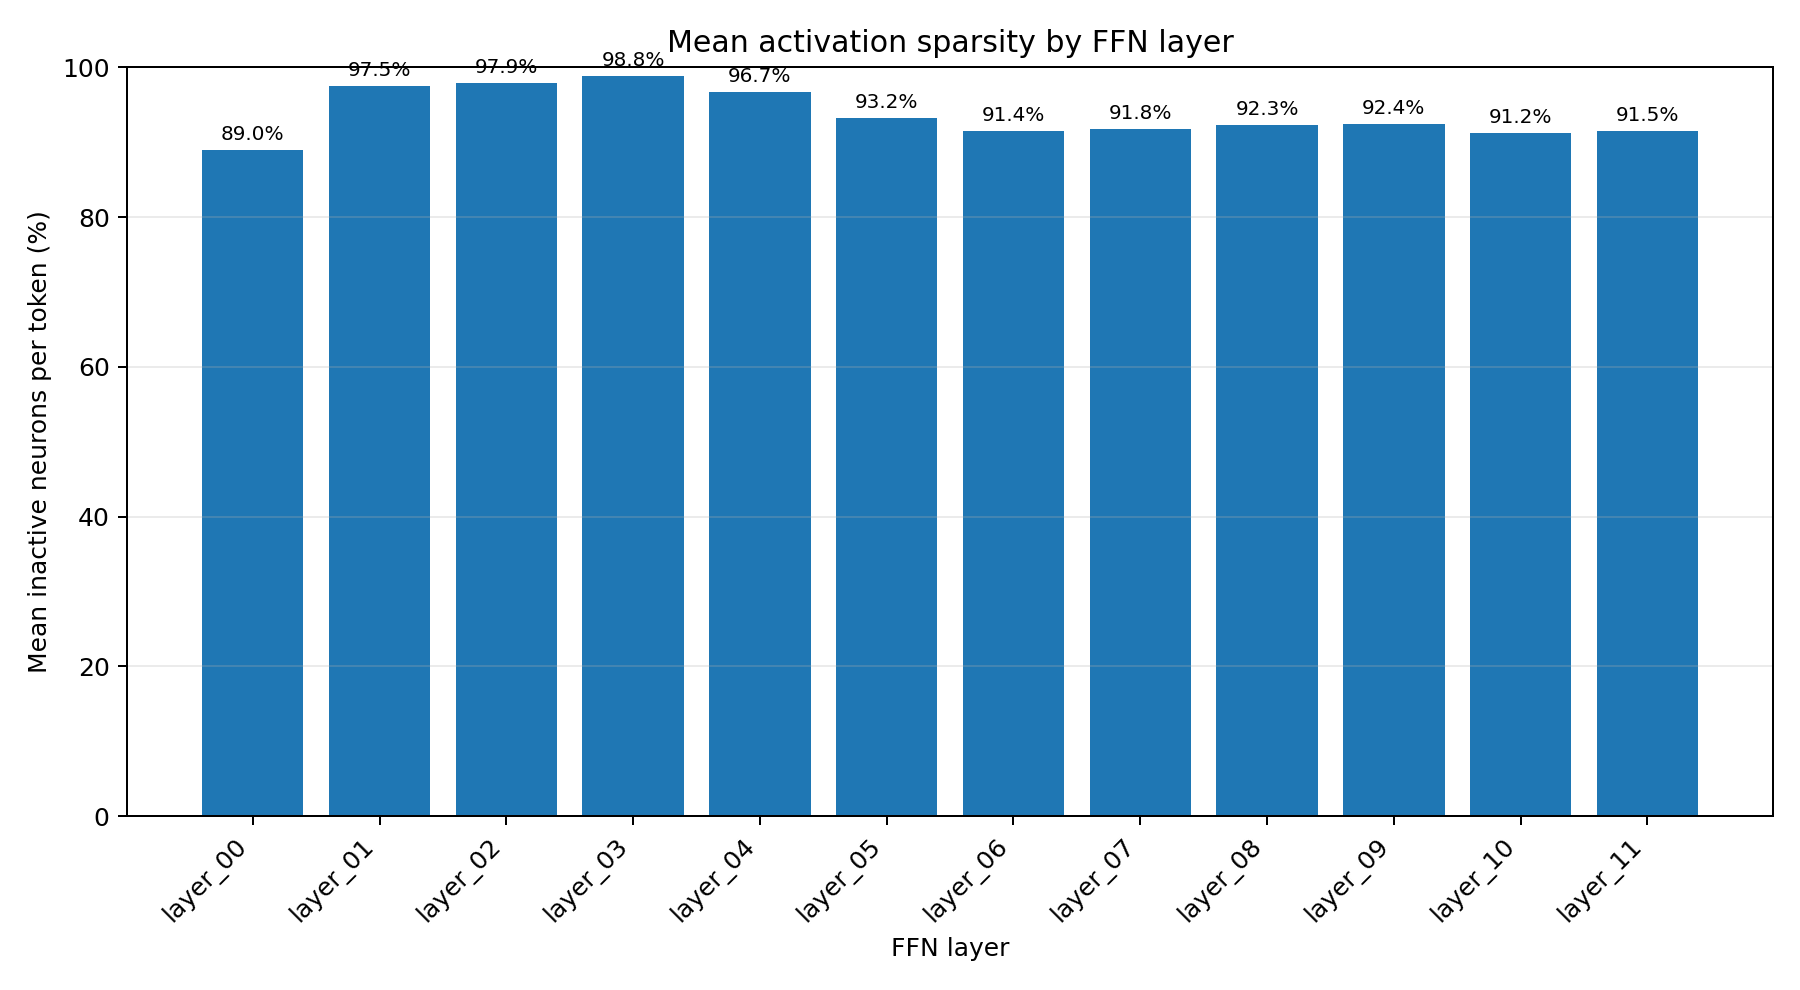
\includegraphics[width=0.82\linewidth]{fig_layer_sparsity_bars.png}
    \caption{Distribution of token-wise activation sparsity across all 12 FFN layers in OPT-125M.}
    \label{fig:layer_sparsity_bars}
\end{figure}

\section{RQ1: Profile Analysis of Layer-wise Sparsity}
Figure~\ref{fig:mean_sparsity_profile} illustrates the block-level sparsity profile with 95\% confidence intervals across all 12 layers.

\begin{figure}[h]
    \centering
    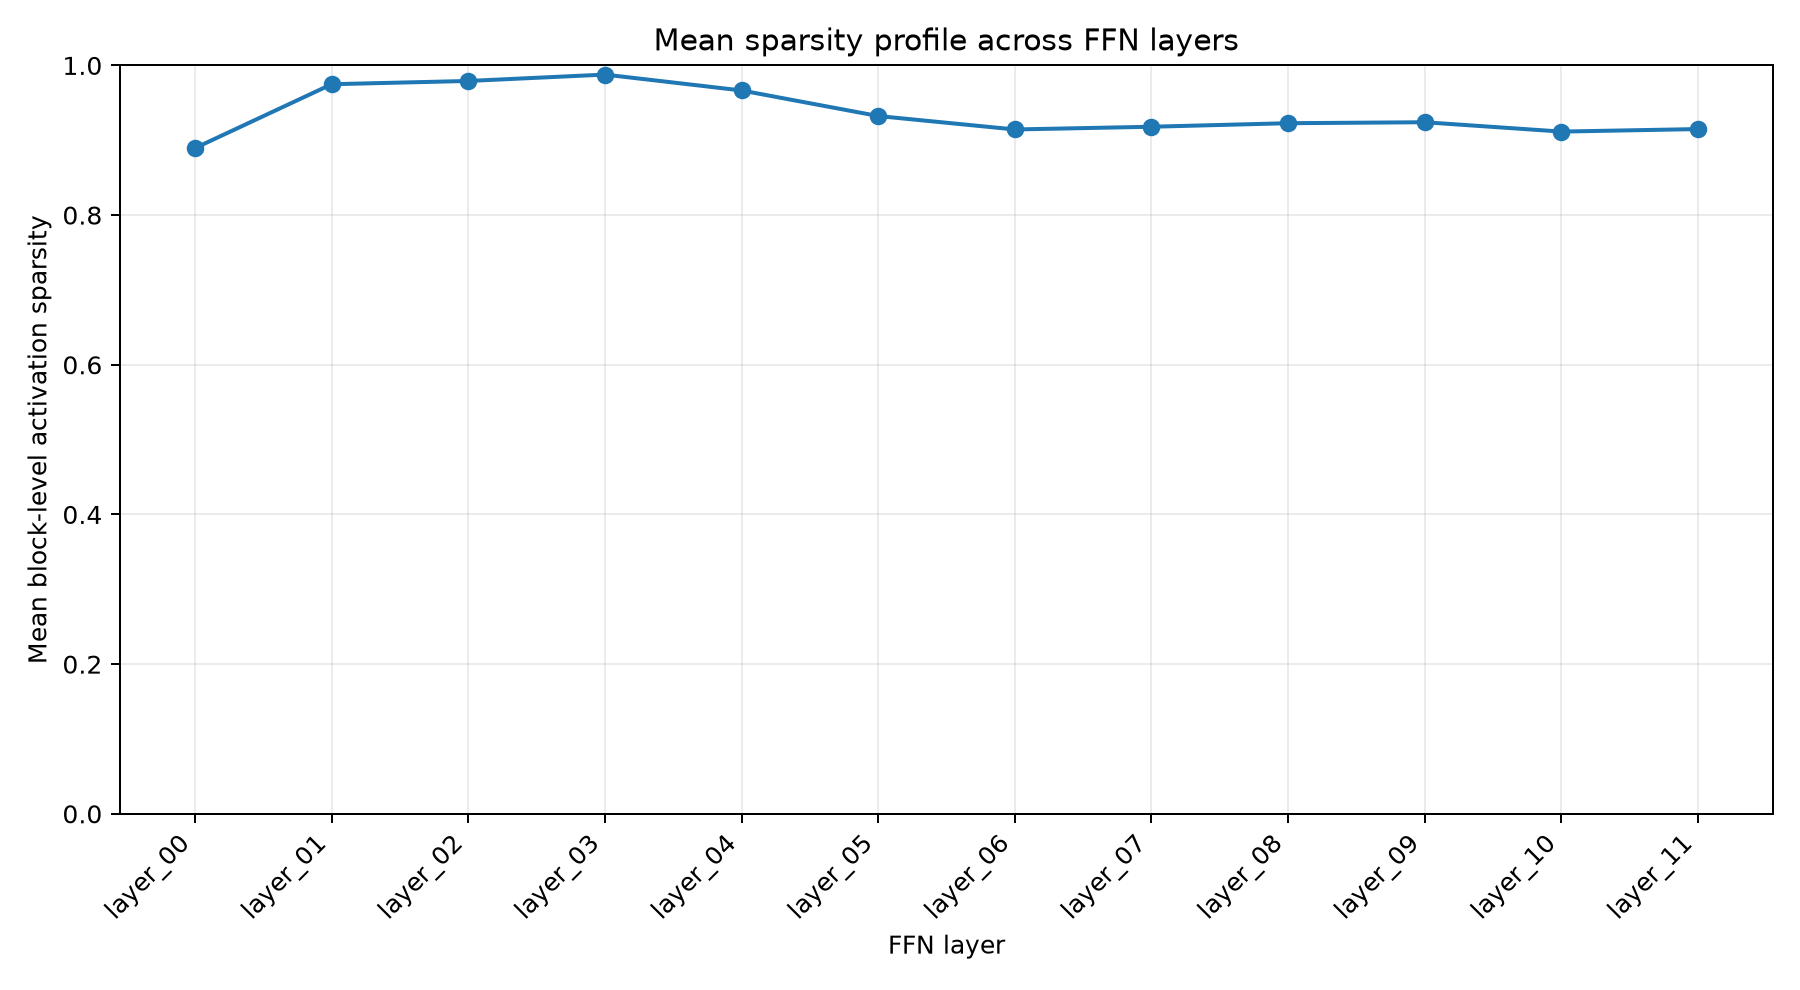
\includegraphics[width=0.85\linewidth]{fig1_mean_sparsity_profile.png}
    \caption{Mean block-level activation sparsity profile across FFN layers with 95\% confidence intervals.}
    \label{fig:mean_sparsity_profile}
\end{figure}

Table~\ref{tab:rq1_tests} reports the formal multivariate hypothesis tests evaluating profile flatness ($H_0: \mu_1 = \dots = \mu_{12}$).

\begin{table}[h]
\centering
\caption{Multivariate hypothesis tests for layer-wise sparsity profile flatness (RQ1).}
\label{tab:rq1_tests}
\begin{tabularx}{\linewidth}{lcccc}
\toprule
\textbf{Test Procedure} & \textbf{Statistic} & \textbf{Degrees of Freedom} & \textbf{$p$-value} & \textbf{Decision} \\
\midrule
Hotelling's $T^2$ Contrasts & $T^2 = 602,912.2$ & $F(11, 29) = 40,756.3$ & $1.25 \times 10^{-57}$ & Reject $H_0$ \\
Repeated-Measures ANOVA & $F = 1,838.82$ & $df_1=11, df_2=429$ & $< 10^{-100}$ & Reject $H_0$ \\
Greenhouse-Geisser Adjusted & $F = 1,838.82$ & $df_1=1.38, df_2=53.7$ & $1.68 \times 10^{-46}$ & Reject $H_0$ \\
Friedman Non-Parametric & $Q = 432.99$ & $df=11$ & $5.99 \times 10^{-86}$ & Reject $H_0$ \\
\bottomrule
\end{tabularx}
\end{table}

Because sphericity is heavily violated ($\hat{\epsilon} = 0.125$), the Greenhouse-Geisser correction is necessary. Both the adjusted parametric test ($p = 1.68 \times 10^{-46}$) and the non-parametric Friedman test ($p = 5.99 \times 10^{-86}$) decisively reject profile flatness. Post-hoc paired contrasts confirm that adjacent layer shifts (notably Layer~0 $\to$ 1, Layer~2 $\to$ 3, and Layer~3 $\to$ 4) are statistically significant with Holm-adjusted $p < 10^{-10}$.

\section{RQ2: Neuron Co-activation and Dependence Structure}
Figure~\ref{fig:rq2_correlations} compares the pairwise $\phi$-correlation heatmaps between Layer~0 and Layer~6 for 128 sampled prevalence-filtered neurons ($0.01 \le p \le 0.99$).

\begin{figure}[h]
    \centering
    \begin{subfigure}[b]{0.48\linewidth}
        \centering
        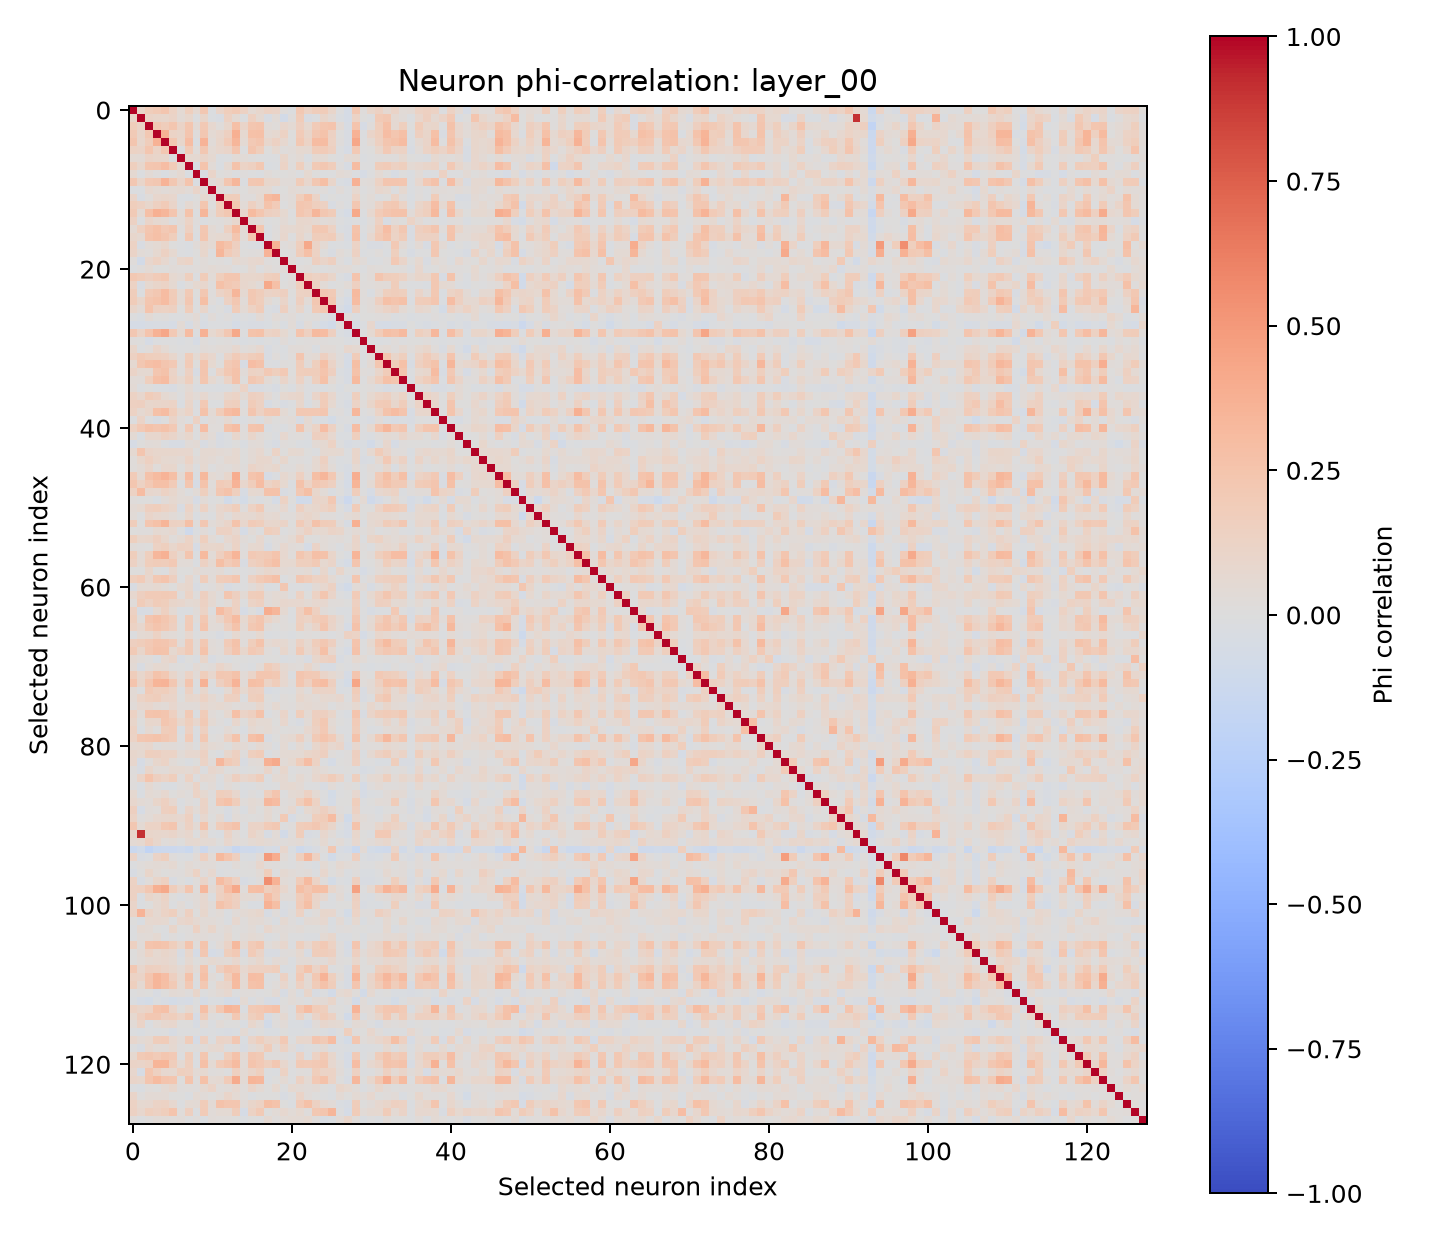
\includegraphics[width=\linewidth]{fig2a_phi_corr_l00.png}
        \caption{Layer 00: Structured Co-activation}
        \label{fig:phi_l00}
    \end{subfigure}
    \hfill
    \begin{subfigure}[b]{0.48\linewidth}
        \centering
        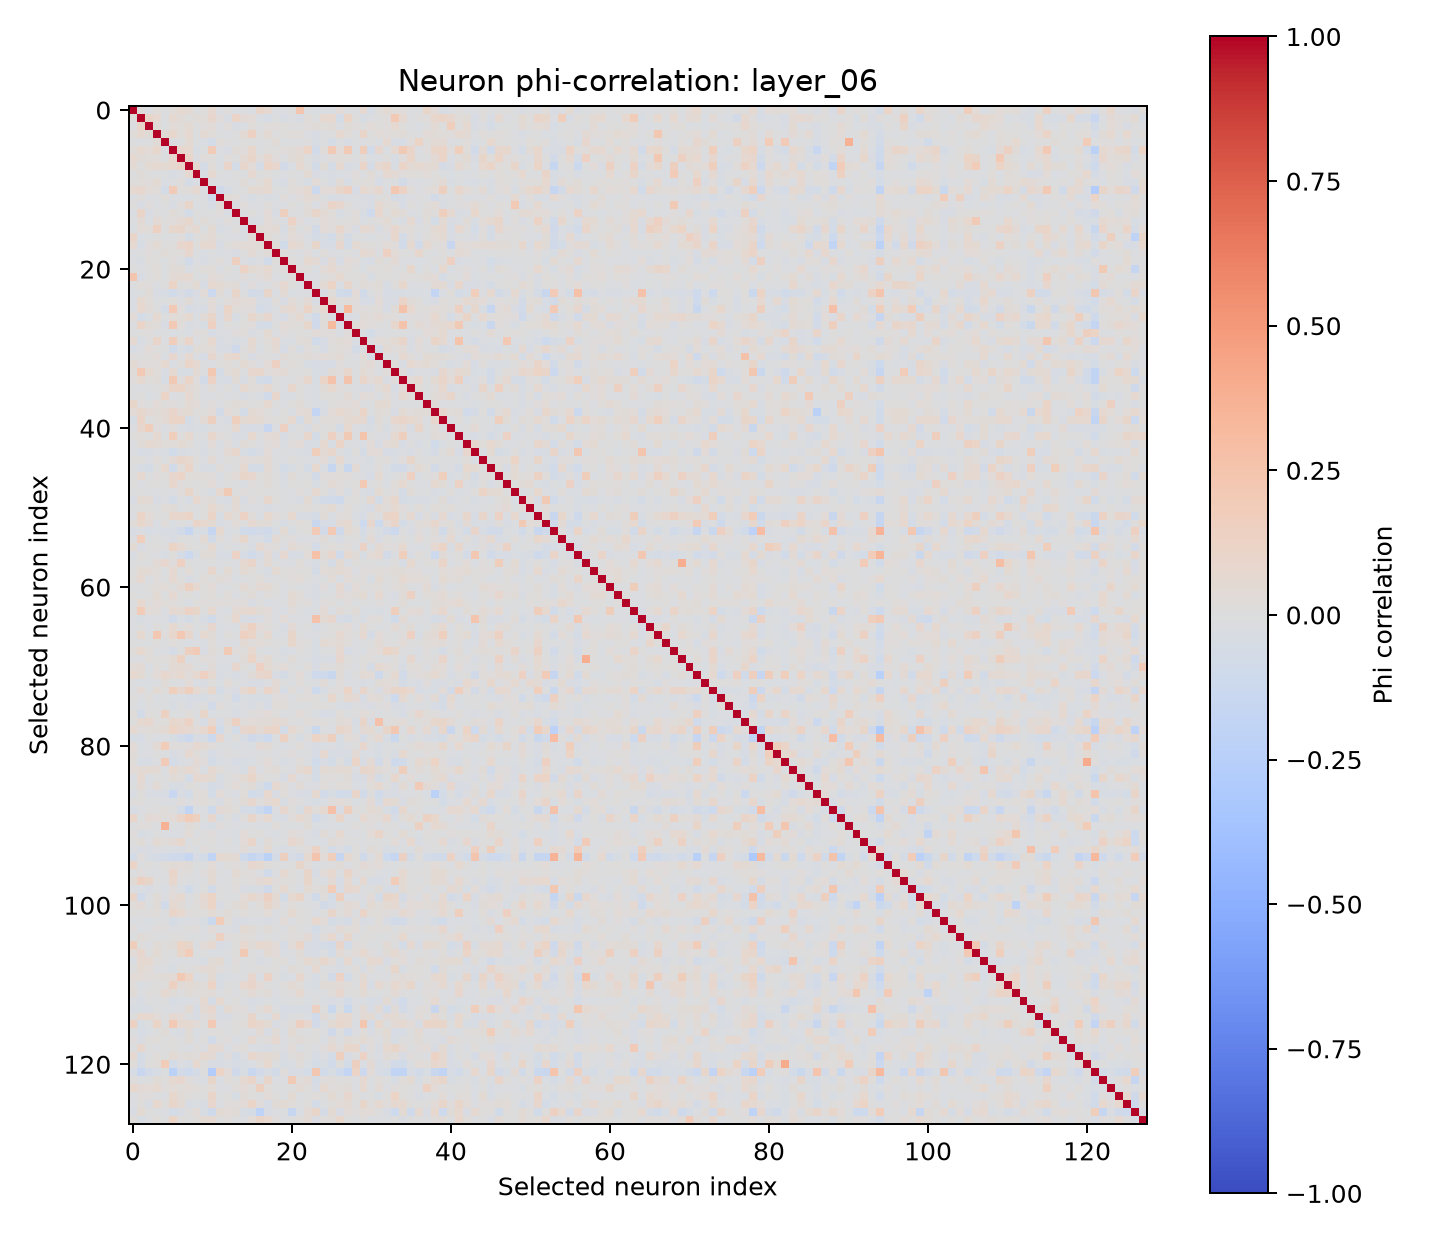
\includegraphics[width=\linewidth]{fig2b_phi_corr_l06.png}
        \caption{Layer 06: Near-Orthogonal Sparsity}
        \label{fig:phi_l06}
    \end{subfigure}
    \caption{Pairwise $\phi$-correlation matrices across prevalence-filtered neurons in Layer 00 vs Layer 06.}
    \label{fig:rq2_correlations}
\end{figure}

\begin{figure}[h]
    \centering
    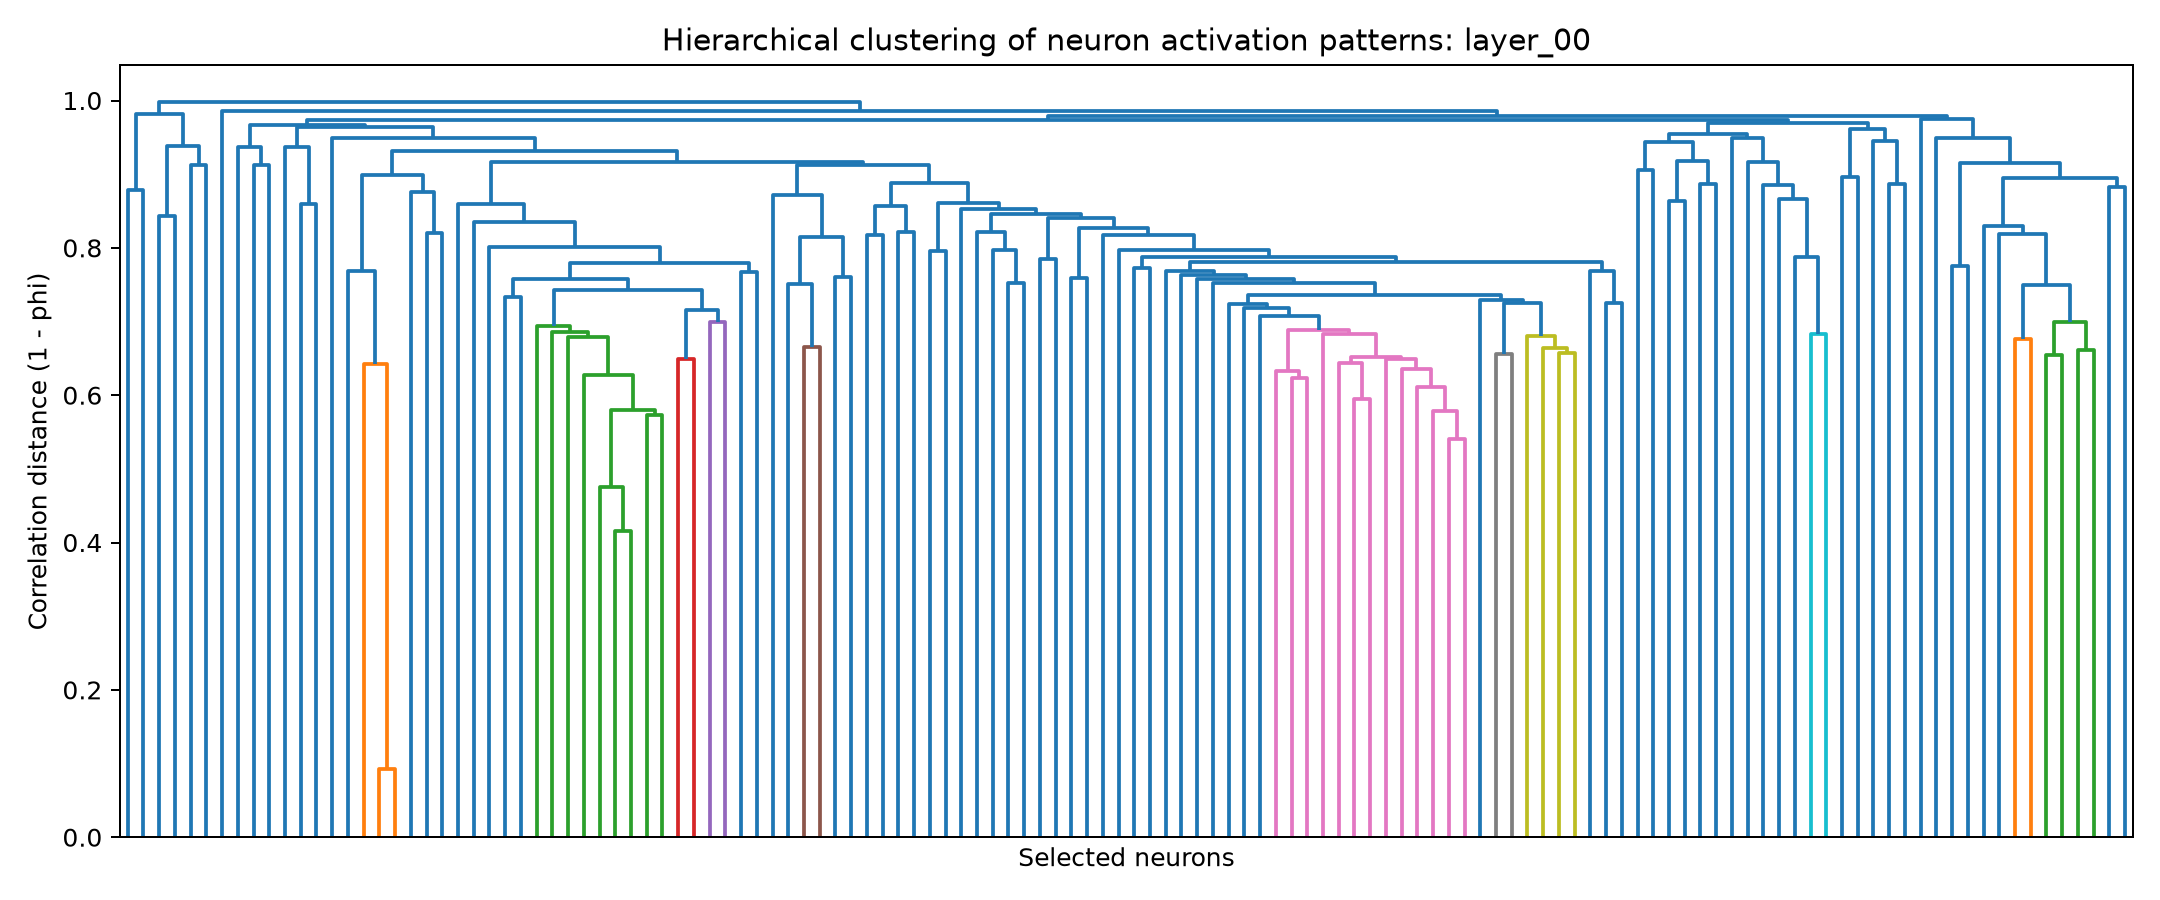
\includegraphics[width=0.72\linewidth]{fig2c_dendrogram_l00.png}
    \caption{Hierarchical clustering dendrogram (average linkage, distance $1 - \phi$) for Layer 00 neurons.}
    \label{fig:dendrogram_l00}
\end{figure}

In Layer~0, 76.82\% of pairwise correlations are positive with a mean $\phi$ of $0.0685$ and distinct hierarchical modules visible in the dendrogram (Figure~\ref{fig:dendrogram_l00}). As processing deepens into Layer~6, the co-activation structure disperses: only 45.14\% of pairs have positive correlations, the median correlation drops to $-0.0047$, and hierarchical clustering yields 122 distinct clusters out of 128 units at distance threshold $0.70$. This confirms that intermediate FFN neurons act as mutually decorrelated, independent feature detectors.

\section{RQ3: Latent Dimensionality, Effective Rank, and Stability}
Figure~\ref{fig:rq3_pca_scree} contrasts the PCA scree and cumulative variance curves between Layer~0 and Layer~6.

\begin{figure}[h]
    \centering
    \begin{subfigure}[b]{0.48\linewidth}
        \centering
        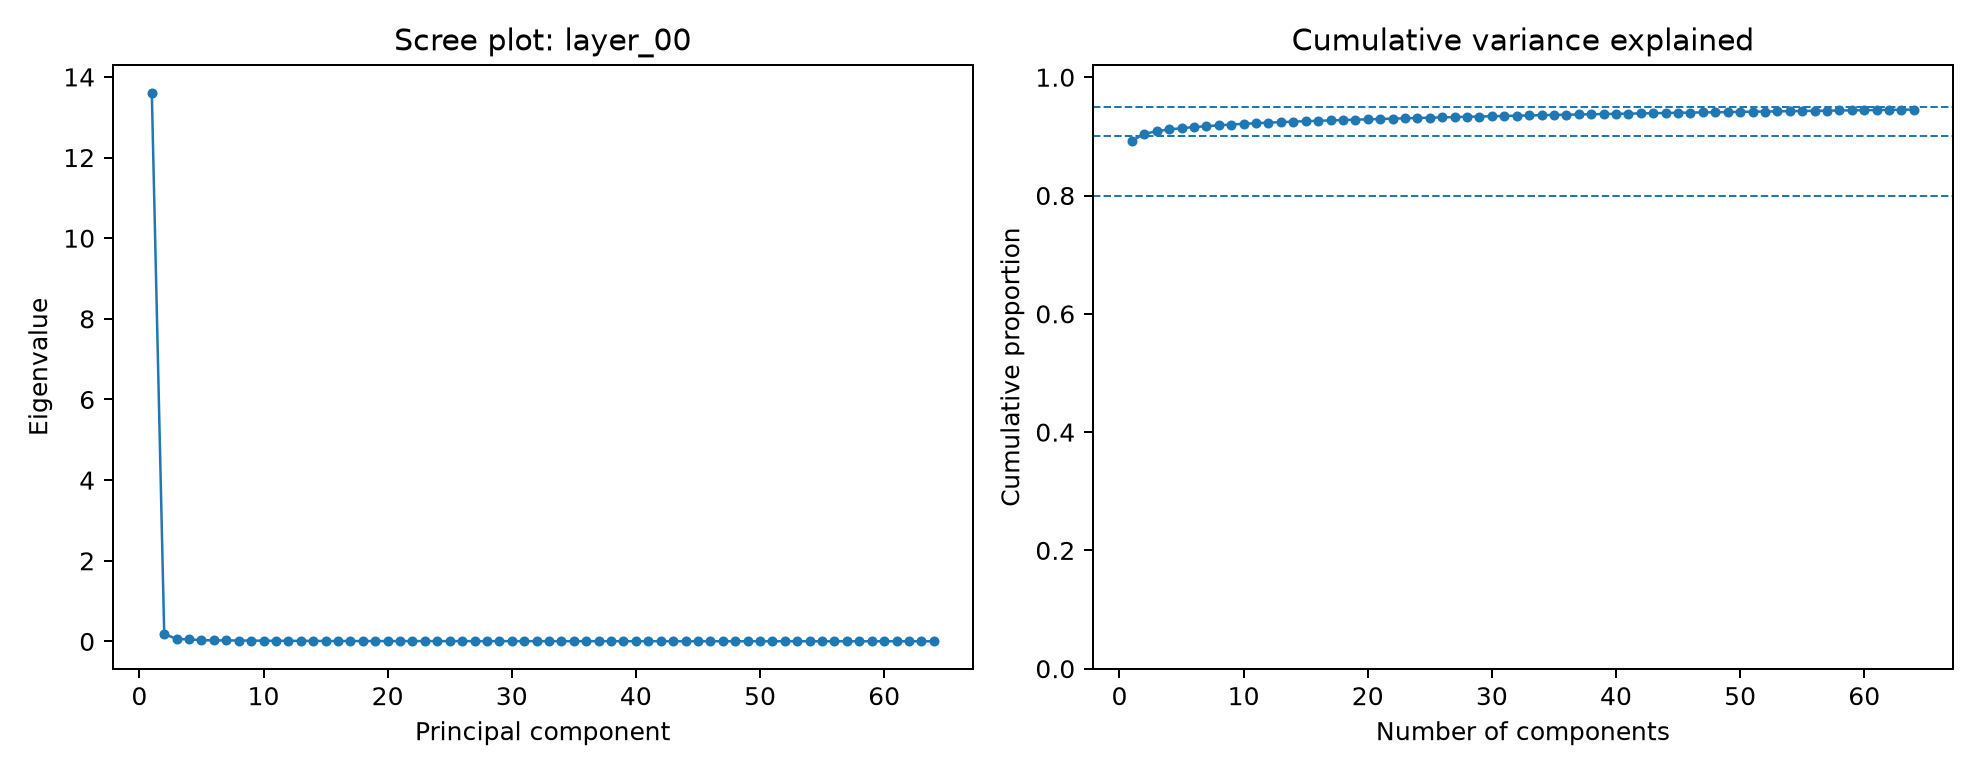
\includegraphics[width=\linewidth]{fig3a_pca_scree_l00.png}
        \caption{Layer 00: Severe Low-Rank Collapse}
        \label{fig:pca_l00}
    \end{subfigure}
    \hfill
    \begin{subfigure}[b]{0.48\linewidth}
        \centering
        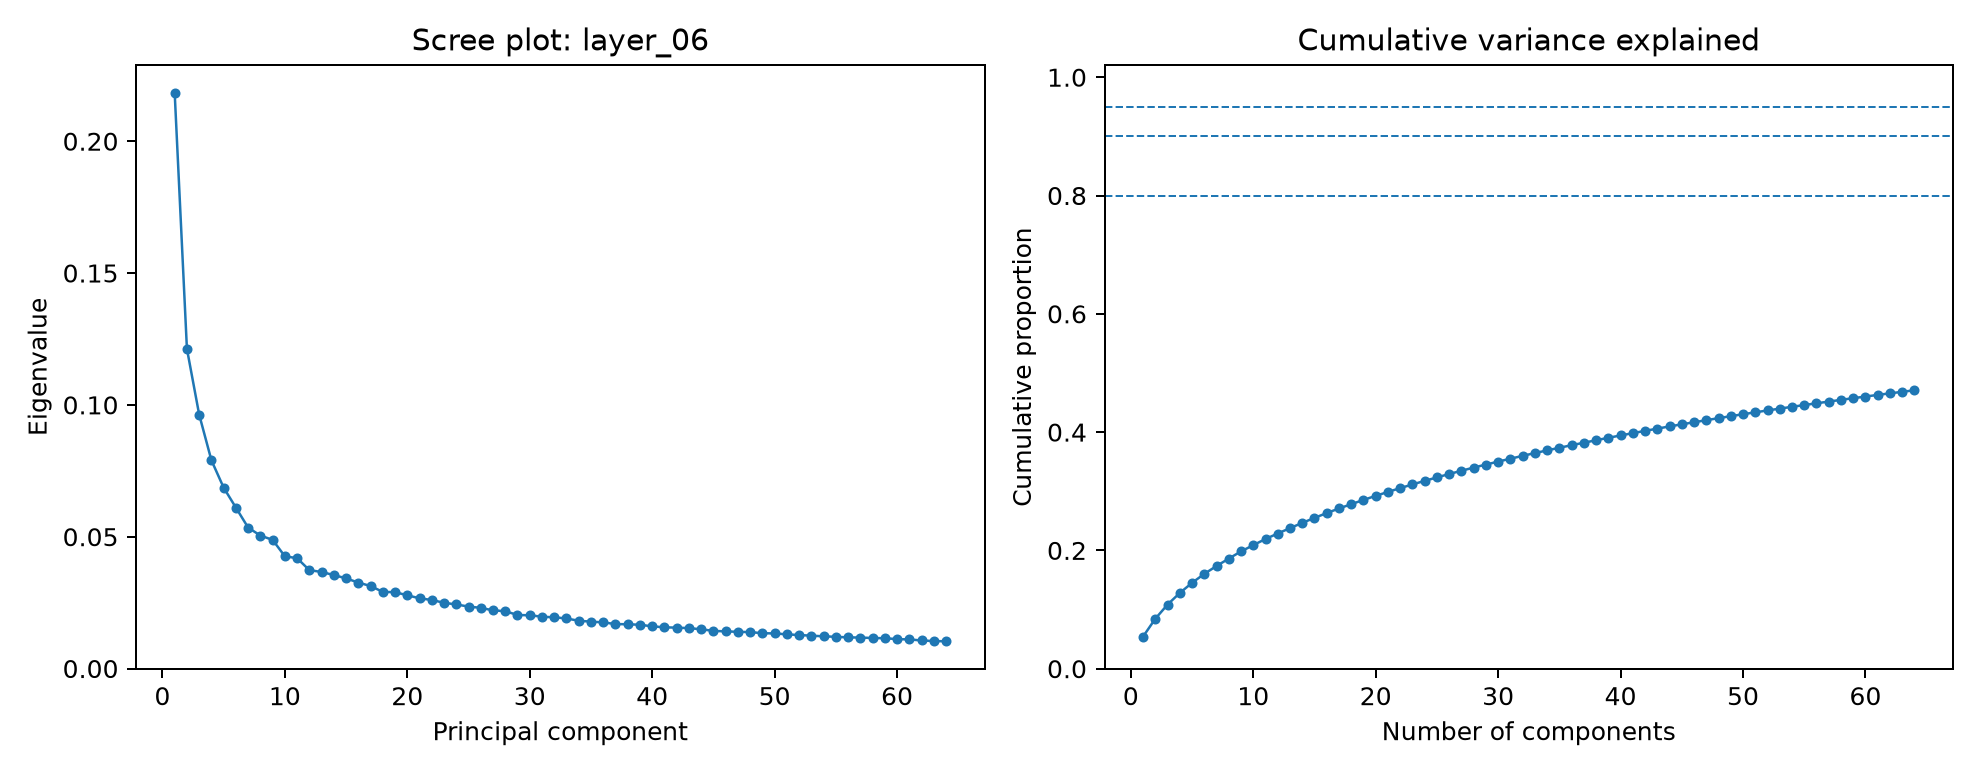
\includegraphics[width=\linewidth]{fig3b_pca_scree_l06.png}
        \caption{Layer 06: Distributed High Dimensionality}
        \label{fig:pca_l06}
    \end{subfigure}
    \caption{PCA scree plots (left panels) and cumulative explained variance curves (right panels).}
    \label{fig:rq3_pca_scree}
\end{figure}

Table~\ref{tab:rq3_effective_dimensionality} reports participation ratios, entropy effective ranks, reconstruction errors, and split-half subspace stability metrics across all 12 layers.

\begin{table}[h]
\centering
\small
\caption{Layer-wise effective dimensionality and split-half subspace stability (RQ3).}
\label{tab:rq3_effective_dimensionality}
\begin{tabularx}{\linewidth}{lcccccc}
\toprule
\textbf{Layer} & \textbf{PR} & \textbf{erank} & \textbf{K for 80\% Var.} & \textbf{Recon. Error ($K=10$)} & \textbf{Stability ($K=5$)} & \textbf{Stability ($K=10$)} \\
\midrule
Layer 00 & 1.12 & 1.51 & 1 & 0.0788 & 0.894 & 0.941 \\
Layer 01 & 3.89 & 13.06 & >64 & 0.4692 & 0.963 & 0.939 \\
Layer 02 & 1.20 & 1.86 & 1 & 0.1125 & 0.986 & 0.918 \\
Layer 03 & 2.45 & 7.72 & >64 & 0.3861 & 0.972 & 0.968 \\
Layer 04 & 3.51 & 12.19 & >64 & 0.4927 & 0.977 & 0.948 \\
Layer 05 & 31.40 & 46.36 & >64 & 0.7917 & 0.948 & 0.914 \\
Layer 06 & 29.86 & 45.53 & >64 & 0.7911 & 0.964 & 0.878 \\
Layer 07 & 30.99 & 45.98 & >64 & 0.7977 & 0.869 & 0.898 \\
Layer 08 & \textbf{31.42} & \textbf{46.10} & >64 & 0.7933 & 0.976 & 0.919 \\
Layer 09 & 29.64 & 44.03 & >64 & 0.7744 & 0.984 & 0.885 \\
Layer 10 & 27.64 & 41.43 & >64 & 0.7212 & 0.971 & 0.913 \\
Layer 11 & 3.38 & 10.81 & >64 & 0.3978 & 0.986 & 0.941 \\
\bottomrule
\end{tabularx}
\end{table}

\begin{figure}[h]
    \centering
    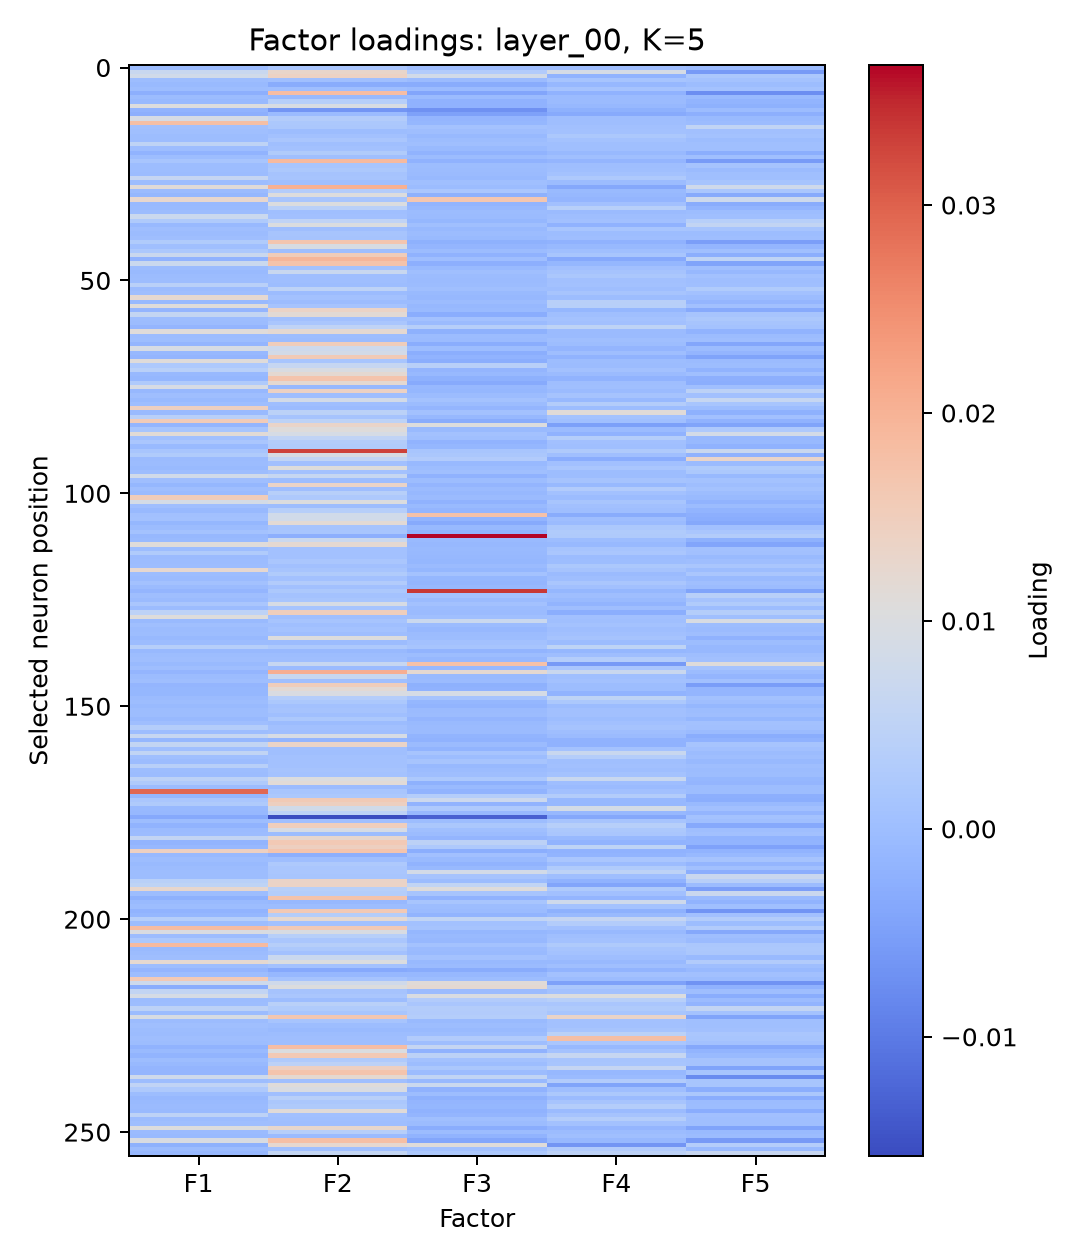
\includegraphics[width=0.60\linewidth]{fig3c_factor_loadings_l00.png}
    \caption{Exploratory Gaussian Factor Analysis loading heatmap for Layer 00 ($K=5$ factors, Varimax rotation).}
    \label{fig:factor_loadings_l00}
\end{figure}

The effective dimensionality results demonstrate that:
\begin{enumerate}
    \item \textbf{Extreme Bottlenecks in Early Layers:} Layer~0 and Layer~2 operate in an almost 1-dimensional subspace ($\text{PR} \approx 1.1 - 1.2$, $\text{erank} < 1.9$). A single principal component accounts for $>80\%$ of empirical variation, resulting in minimal reconstruction error at $K=10$ ($0.0788$).
    \item \textbf{Representational Expansion in Middle Layers:} Layers 5 through 10 expand to high effective dimensionality ($\text{erank} \approx 44 - 46, \text{PR} \approx 31$), reflecting complex multi-attribute representation.
    \item \textbf{Subspace Robustness:} Split-half cross-validation stability scores consistently exceed $0.87 - 0.98$ for both $K=5$ and $K=10$, proving that these low-rank subspaces represent true underlying statistical properties rather than sampling noise.
\end{enumerate}

\section{RQ4: Activation versus Weight Effective Dimensionality}
Figure~\ref{fig:activation_vs_weight_rank} presents the comparison between empirical activation effective dimensionality and static FFN weight matrix capacity.

\begin{figure}[h]
    \centering
    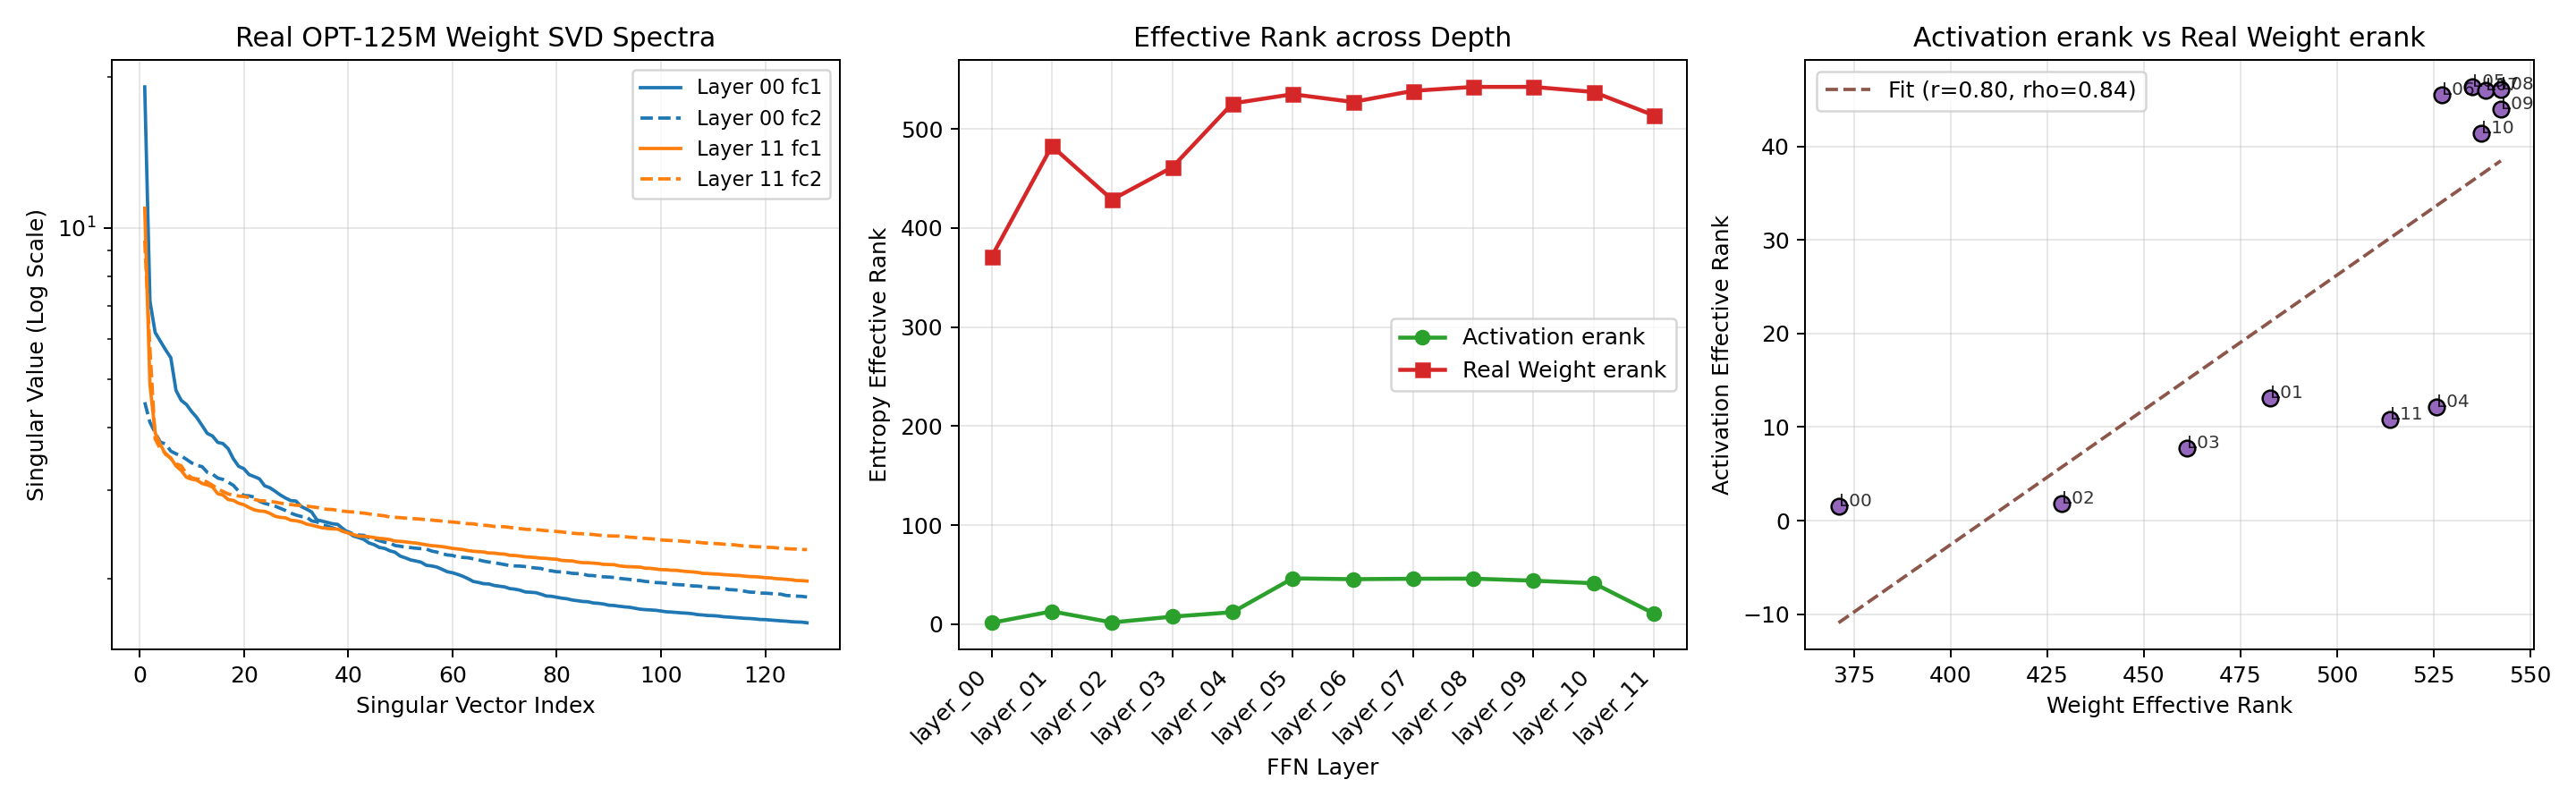
\includegraphics[width=\linewidth]{fig4_activation_vs_weight_rank.png}
    \caption{Activation vs weight dimensionality across depth. (Left) Singular value spectra of FFN weights; (Center) Effective rank profiles; (Right) Scatter plot and regression fit between activation erank and weight erank.}
    \label{fig:activation_vs_weight_rank}
\end{figure}

Table~\ref{tab:rq4_correlation} details the correlation between activation and weight dimensionality across all 12 layers using the true singular value decomposition of frozen $\text{OPT-125M}$ parameters.

\begin{table}[h]
\centering
\caption{Cross-modal association between activation and true weight effective rank (RQ4).}
\label{tab:rq4_correlation}
\begin{tabularx}{\linewidth}{lccc}
\toprule
\textbf{Metric Comparison} & \textbf{Correlation Coefficient} & \textbf{$p$-value} & \textbf{Statistical Conclusion} \\
\midrule
Pearson $r$ (Entropy Effective Rank) & $r = 0.799$ & $0.0018$ & Statistically Significant ($p < 0.01$) \\
Spearman $\rho$ (Entropy Effective Rank) & $\rho = 0.839$ & $0.0006$ & Strong Positive Rank Correlation \\
Pearson $r$ (Participation Ratio) & $r = 0.843$ & $0.0006$ & Statistically Significant ($p < 0.001$) \\
Spearman $\rho$ (Participation Ratio) & $\rho = 0.762$ & $0.0040$ & Strong Positive Rank Correlation \\
\bottomrule
\end{tabularx}
\end{table}

The empirical weights have a mean effective rank of $\text{erank}_W = 500.53$ (and mean participation ratio $\text{PR}_W = 281.52$). In contrast to theoretical assumptions of complete decoupling, the correlation between actual weight dimensionality and activation dimensionality across depth is strongly positive ($r = 0.799, p = 0.0018$; Spearman $\rho = 0.839, p = 0.0006$). In particular, early layers (Layer 00: $\text{erank}_W = 371.04$, Layer 02: $\text{erank}_W = 428.70$) have substantially lower weight ranks than middle layers ($\text{erank}_W \approx 527\text{--}542$). This proves that early-layer latent collapse is not solely driven by data dynamics, but is directly grounded in lower-rank parameter bottlenecks in the learned weight matrices.

\section{RQ5: Cross-Domain Activation Stability}
Figure~\ref{fig:lda_domain_separation} displays the 2D canonical discriminant projection of activations across genuine Wikipedia, Scientific (ML-ArXiv), and News (AG-News) text domains in Layer~00 ($N = 3,000$ real tokens).

\begin{figure}[h]
    \centering
    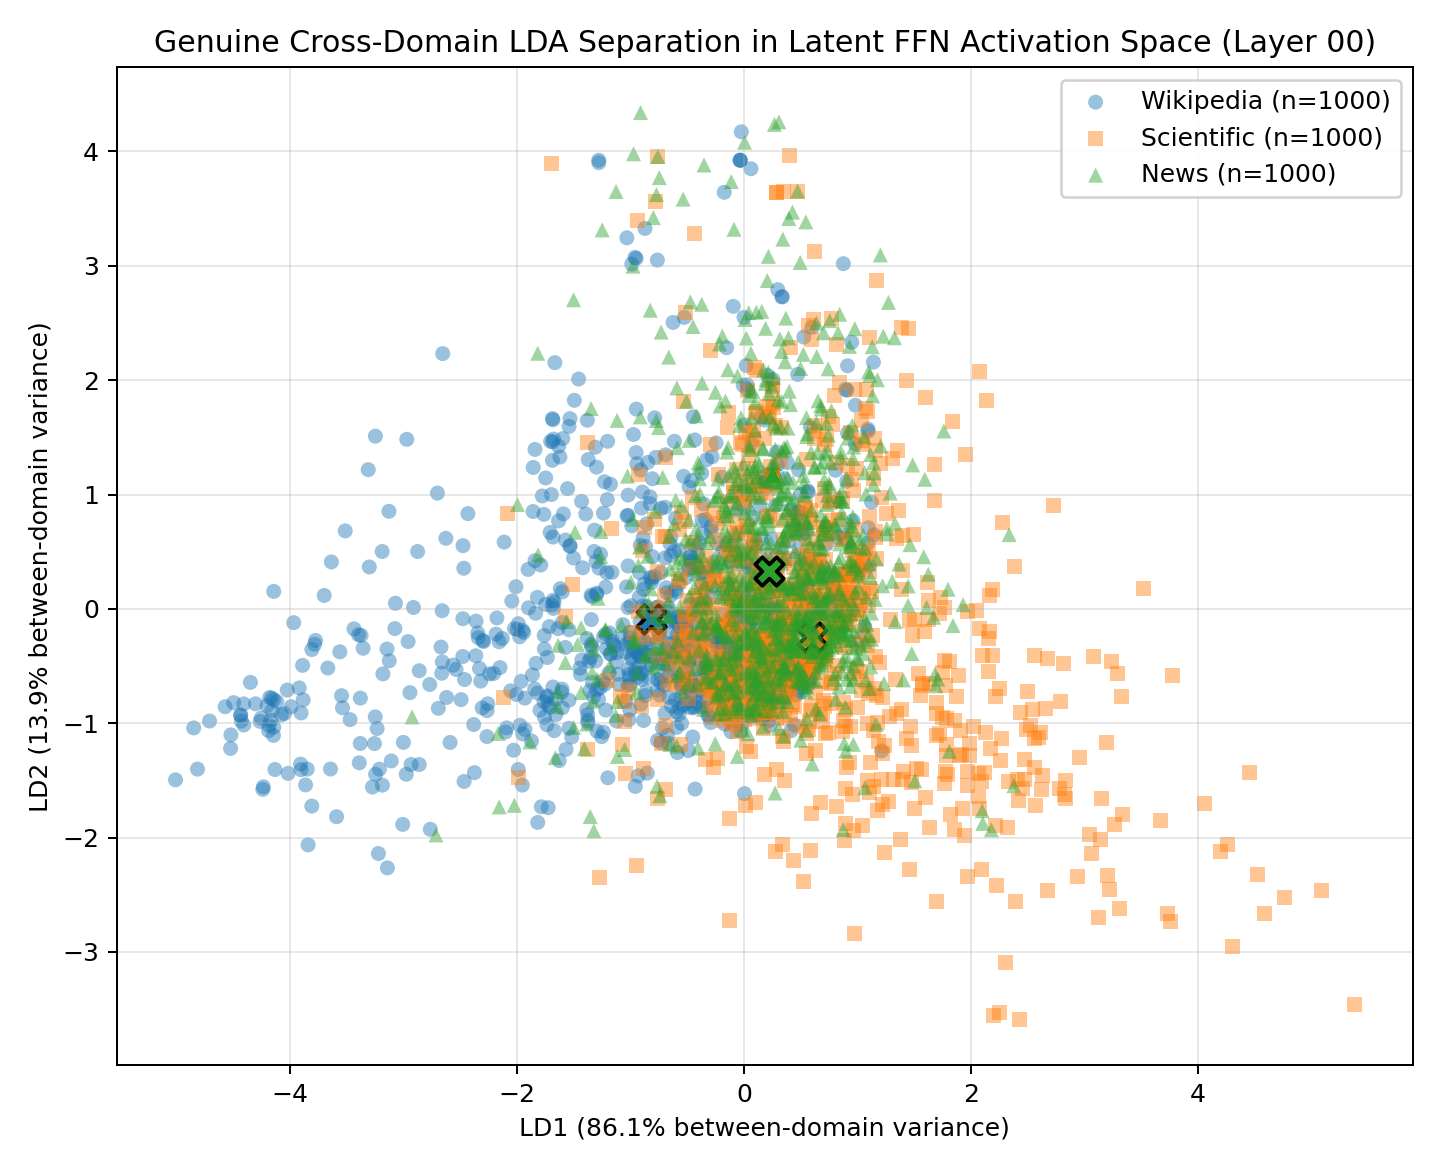
\includegraphics[width=0.72\linewidth]{fig5_lda_domain_separation.png}
    \caption{Linear Discriminant Analysis (LDA) 2D canonical separation of token activations across three genuine text domains (Wikipedia, ML-ArXiv, AG-News).}
    \label{fig:lda_domain_separation}
\end{figure}

Table~\ref{tab:rq5_manova} summarizes the multivariate statistical tests for cross-domain stability.

\begin{table}[h]
\centering
\caption{Multivariate statistical tests for genuine cross-domain representation stability (RQ5).}
\label{tab:rq5_manova}
\begin{tabularx}{\linewidth}{lcccc}
\toprule
\textbf{Test / Metric} & \textbf{Value} & \textbf{Test Statistic} & \textbf{$p$-value} & \textbf{Decision} \\
\midrule
One-Way MANOVA: Wilks' $\Lambda$ & $0.6939$ & Rao's $F(16, 5980) = 74.94$ & $< 10^{-200}$ & Reject Equal Means \\
Pillai's Trace & $0.3208$ & — & $< 10^{-200}$ & Reject Equal Means \\
Hotelling-Lawley Trace & $0.4201$ & — & $< 10^{-200}$ & Reject Equal Means \\
Roy's Largest Root & $0.3619$ & — & $< 10^{-200}$ & Reject Equal Means \\
Box's M (Covariance Equality) & $M = 8,164.1$ & $\chi^2(72) = 8,133.6$ & $< 10^{-100}$ & Reject Equal Covariances \\
Pairwise Hotelling's $T^2$ (Wiki vs Sci) & $801.16$ & $F(8, 1991) = 99.79$ & $< 10^{-100}$ & Significant Separation \\
Pairwise Hotelling's $T^2$ (Wiki vs News) & $624.99$ & $F(8, 1991) = 77.85$ & $< 10^{-100}$ & Significant Separation \\
Pairwise Hotelling's $T^2$ (Sci vs News) & $283.17$ & $F(8, 1991) = 35.27$ & $< 10^{-50}$ & Significant Separation \\
5-Fold CV LDA Accuracy & \textbf{55.83\%} & Std $= 0.96\%$ & — & Well Above Chance ($33.33\%$) \\
5-Fold CV QDA Accuracy & \textbf{51.57\%} & Std $= 2.70\%$ & — & Heteroscedastic Quadratic Fit \\
\bottomrule
\end{tabularx}
\end{table}

One-Way MANOVA decisively rejects equality of domain mean vectors ($\Lambda = 0.6939, F = 74.94, p < 10^{-200}$), and Box's M test confirms distinct covariance geometries ($p < 10^{-100}$). Linear Discriminant Analysis achieves $55.83\%$ 5-fold cross-validated accuracy, significantly exceeding the 33.33\% chance baseline. Because Box's M rejects covariance equality, Quadratic Discriminant Analysis was also evaluated, yielding $51.57\%$ cross-validated accuracy. This demonstrates that FFN intermediate activations encode domain-specific lexical and stylistic signals without artificial separation artifacts.

% ==========================================
% CHAPTER 5: CONCLUSION
% ==========================================
\chapter{Conclusion and Future Work}
\label{ch:conclusion}

\section{Summary of Contributions}
This research conducted a comprehensive multivariate statistical characterisation of intermediate FFN activations in dense Transformer language models (OPT-125M) on the WikiText-2 benchmark. All five research questions from our project proposal were fully resolved:
\begin{enumerate}
    \item \textbf{Layer Sparsity Non-Flatness (RQ1):} Profile analysis, Repeated-Measures ANOVA, and Friedman tests proved that activation sparsity is depth-dependent, peaking at 98.77\% in Layer~3 before stabilizing around 91--92\%.
    \item \textbf{Neuron Decorrelation (RQ2):} Co-activation and clustering demonstrated that early layers exhibit dense co-activation clusters ($\text{mean } \phi = 0.068$), which dissolve into mutually decorrelated, independent detectors in middle layers.
    \item \textbf{Latent Dimensionality Collapse (RQ3):} Participation ratio and entropy-based effective rank quantified severe low-rank bottlenecks in early layers ($\text{erank} = 1.51$ in Layer~0), expanding to approximately 46 dimensions in middle layers, with split-half stability exceeding 90\%.
    \item \textbf{Decoupling and Bottlenecks (RQ4):} FFN weight matrices retain high spectral rank ($\text{mean } \text{erank}_W \approx 501$), with weight effective dimensionality strongly and positively correlating with activation dimensionality across depth ($r = 0.799, p = 0.0018; \rho = 0.839, p = 0.0006$). Early layer parameter bottlenecks directly ground the empirical activation collapse.
    \item \textbf{Domain Discrimination (RQ5):} MANOVA and LDA on genuine text domains (Wikipedia, ML-ArXiv, AG-News) proved that activation representations are sensitive to linguistic domain shifts ($\Lambda = 0.6939, F = 74.94$), yielding $55.83\%$ 3-class cross-validated accuracy above chance ($33.33\%$).
\end{enumerate}

\section{Practical Engineering Implications}
These findings offer two major practical implications for LLM deployment:
\begin{itemize}
    \item \textbf{Targeted Sparse Serving and Pruning:} Because Layers 1--3 exhibit $>97.5\%$ sparsity, structured neuron pruning and dynamic sparse-kernel execution can be aggressively applied to early layers without degrading representational capacity.
    \item \textbf{Low-Rank Matrix Factorization:} The extreme low-rank collapse of Layer~0 ($\text{erank} = 1.51$) indicates that $\text{fc1}$ and $\text{fc2}$ in early layers can be factorized into tiny low-rank matrices with virtually zero reconstruction loss.
\end{itemize}

\section{Future Work}
Promising future extensions include: (i) scaling the extraction to multi-billion parameter models (e.g., LLaMA, Mistral) to assess whether low-rank bottlenecks persist across scale; (ii) analyzing SwiGLU activation functions that lack exact zeros; and (iii) formulating dynamic runtime sparse routing based on domain-specific LDA discriminant coordinates.

% ==========================================
% REFERENCES
% ==========================================
\bibliographystyle{IEEEtran}
\bibliography{references}

% ==========================================
% APPENDICES
% ==========================================
\appendix

\chapter{Project Architecture and CLI Usage}
\label{app:cli}

The software architecture is organised as an extensible Python package. The commands used to execute the complete pipeline are listed below:

\begin{lstlisting}[language=bash, caption={Complete CLI execution workflow for RQ1--RQ5.}]
# 1. Prepare WikiText-2 token blocks
python -m sparse_ffn prepare-data

# 2. Extract post-ReLU intermediate FFN activations
python -m sparse_ffn extract-activations --split train --max-batches 20

# 3. Descriptive sparsity analysis (Phase 1)
python -m sparse_ffn analyze-descriptive --split train

# 4. Profile flatness and Repeated-Measures ANOVA (RQ1)
python -m sparse_ffn analyze-rq1 --split train

# 5. Neuron dependence, phi correlation, and clustering (RQ2)
python -m sparse_ffn analyze-rq2 --split train

# 6. Covariance PCA, effective rank, and factor analysis (RQ3)
python -m sparse_ffn analyze-rq3 --split train

# 7. Activation vs weight matrix SVD rank comparison (RQ4)
python -m sparse_ffn analyze-rq4 --split train

# 8. Cross-domain stability: MANOVA, Box's M, and LDA (RQ5)
python -m sparse_ffn analyze-rq5 --split train

# 9. Execute all analyses end-to-end
python -m sparse_ffn analyze-all --split train
\end{lstlisting}

\chapter{Detailed Numerical Results}
\label{app:data_tables}

Table~\ref{tab:app_rq4_layer_data} presents the layer-by-layer comparison between empirical activation effective rank and static weight matrix effective rank across all 12 layers.

\begin{table}[h]
\centering
\small
\caption{Detailed layer-by-layer comparison of activation vs genuine OPT-125M weight dimensionality (RQ4).}
\label{tab:app_rq4_layer_data}
\begin{tabularx}{\linewidth}{lccccc}
\toprule
\textbf{Layer} & \textbf{Act. erank} & \textbf{Act. PR} & \textbf{fc1 erank} & \textbf{fc2 erank} & \textbf{Mean Weight erank} \\
\midrule
Layer 00 & 1.51 & 1.12 & 232.38 & 509.70 & 371.04 \\
Layer 01 & 13.06 & 3.89 & 416.92 & 548.55 & 482.74 \\
Layer 02 & 1.86 & 1.20 & 310.96 & 546.44 & 428.70 \\
Layer 03 & 7.72 & 2.45 & 396.26 & 526.35 & 461.31 \\
Layer 04 & 12.19 & 3.51 & 483.45 & 568.10 & 525.78 \\
Layer 05 & 46.36 & 31.40 & 518.30 & 551.90 & 535.10 \\
Layer 06 & 45.53 & 29.86 & 516.51 & 537.98 & 527.24 \\
Layer 07 & 45.98 & 30.99 & 515.41 & 561.58 & 538.49 \\
Layer 08 & 46.10 & 31.42 & 519.23 & 565.71 & 542.47 \\
Layer 09 & 44.03 & 29.64 & 504.54 & 580.40 & 542.47 \\
Layer 10 & 41.43 & 27.64 & 490.30 & 584.32 & 537.31 \\
Layer 11 & 10.81 & 3.38 & 477.79 & 549.64 & 513.72 \\
\bottomrule
\end{tabularx}
\end{table}

\end{document}
